\documentclass[10pt,letterpaper]{article}

\usepackage{eso-pic}


\AddToShipoutPictureBG{%

\ifnum\value{page}>1{
\AtTextUpperLeft{
\makebox[18.5cm][r]{
\raisebox{-2.3cm}{%
{\transparent{0.3}{
\includegraphics[width=0.29\textwidth]{e-logo.png}}	}} } }
}\fi
}

\AddToShipoutPicture{%
{
 {\color{blGreen!70!red}\transparent{0.9}{\put(0,0){\rule{3pt}{\paperheight}}}}%
 {\color{darkRed!70!purple}\transparent{1}\put(3,0){{\rule{4pt}{\paperheight}}}}
% {\color{logoPeach!80!cyan}\transparent{0.5}{\put(0,700){\rule{1cm}{.6cm}}}}%
% {\color{darkRed!60!cyan}\transparent{0.7}\put(0,706){{\rule{1cm}{.6cm}}}}
% \put(18,726){\thepage}
% \transparent{0.8}
}
}



\AddToShipoutPicture{%

\ifnum\value{page}>0


{\color{blGreen!70!red}\transparent{0.9}{\put(300,8){\rule{0.5\paperwidth}{.3cm}}}}%
{\color{inOne}\transparent{0.8}{\put(300,10){\rule{0.5\paperwidth}{.3cm}}}}%
{\color{inTwo}\transparent{0.3}\put(300,13){{\rule{0.5\paperwidth}{.3cm}}}}

\put(301,16){%
\transparent{0.7}{

\includegraphics[width=0.2\textwidth]{logo.png}} }

{\color{blGreen!70!red}\transparent{0.9}{\put(5.6,5){\rule{0.5\paperwidth}{.4cm}}}}%
{\color{inOne}\transparent{1}{\put(5.6,10){\rule{0.5\paperwidth}{.4cm}}}}%
{\color{inTwo}\transparent{0.3}\put(5.6,15){{\rule{0.5\paperwidth}{.4cm}}}}

\fi
}

%\pagestyle{empty} % no page number
%\parskip 7.2pt    % space between paragraphs
%\parindent 12pt   % indent for new paragraph
%\textwidth 4.5in  % width of text
%\columnsep 0.8in  % separation between columns

\setlength{\footskip}{23pt}

\usepackage[paperheight=15.5in,paperwidth=9.1in]{geometry}
\geometry{left=1.3in,top=1.1in,right=.6in,bottom=1.6in} %margins

\newcommand{\sectsp}{\vspace{12pt}}

\usepackage{graphicx}
\usepackage{color,framed}

\usepackage{float}

\usepackage{mdframed}


\usepackage{setspace}
\newcommand{\rpdfNotice}[1]{\begin{onehalfspacing}{

\Large #1

}\end{onehalfspacing}}

\usepackage{xcolor}

\usepackage[hyphenbreaks]{breakurl}
\usepackage[hyphens]{url}

\usepackage{hyperref}
\newcommand{\rpdfLink}[1]{\href{#1}{\small{#1}}}
\newcommand{\dblHref}[1]{\href{#1}{\small{\burl{#1}}}}
\newcommand{\browseHref}[2]{\href{#1}{\Large #2}}

\hypersetup{
    colorlinks=true,
    linkcolor=cyan,
    filecolor=magenta,
    urlcolor=blue,
}

\urlstyle{same}

\definecolor{blGreen}{rgb}{.2,.7,.3}
\definecolor{darkRed}{rgb}{.2,.0,.1}

\definecolor{darkBlGreen}{rgb}{.1,.3,.2}

\definecolor{oldBlColor}{rgb}{.2,.7,.3}

\definecolor{blColor}{rgb}{.1,.3,.2}

\definecolor{elColor}{rgb}{.2,.1,0}
\definecolor{flColor}{rgb}{0.7,0.3,0.3}

\definecolor{logoOrange}{RGB}{108, 18, 30}
\definecolor{logoGreen}{RGB}{85, 153, 89}
\definecolor{logoPurple}{RGB}{200, 208, 30}

\definecolor{logoBlue}{RGB}{4, 2, 25}
\definecolor{logoPeach}{RGB}{255, 159, 102}
\definecolor{logoCyan}{RGB}{66, 206, 244}
\definecolor{logoRed}{rgb}{.3,0,0}

\definecolor{inOne}{rgb}{0.122, 0.435, 0.698}% Rule colour
\definecolor{inTwo}{rgb}{0.122, 0.698, 0.435}% Rule colour

\definecolor{outOne}{rgb}{0.435, 0.698, 0.122}% Rule colour
\definecolor{outTwo}{rgb}{0.698, 0.435, 0.122}% Rule colour

\usepackage[many]{tcolorbox}% http://ctan.org/pkg/tcolorbox

\usepackage{transparent}

\newenvironment{cframed}{\begin{mdframed}[linecolor=logoPeach,linewidth=0.4mm]}{\end{mdframed}}

\newenvironment{ccframed}{\begin{mdframed}[backgroundcolor=logoGreen!5,linecolor=logoCyan!50!black,linewidth=0.4mm]}{\end{mdframed}}

\usepackage{aurical}
\usepackage[T1]{fontenc}

\usepackage{relsize}

\newcommand{\pseudoIndent}{

\vspace{10pt}\hspace*{38pt}}

\newcommand{\YPDFI}{{\fontfamily{fvs}\selectfont YPDF-Interactive}}

%
\newcommand{\deconum}[1]{{\protect\raisebox{-1pt}{{\LARGE #1}}}}



\newcommand{\VersatileUX}{{\color{red!85!black}{\Fontauri Versatile}}%
{{\fontfamily{qhv}\selectfont\smaller UX}}}

\newcommand{\NDPCloud}{{\color{red!15!black}%
{\fontfamily{qhv}\selectfont {\smaller NDP C{\smaller LOUD}}}}}

\newcommand{\lfNDPCloud}{{\color{red!15!black}%
{\fontfamily{qhv}\selectfont N{\smaller DP C{\smaller LOUD}}}}}

\newcommand{\textds}[1]{{\fontfamily{lmdh}\selectfont{%
\raisebox{-1pt}{#1}}}}

\newcommand{\dsC}{{\textds{ds}{\fontfamily{qhv}\selectfont \raisebox{-1pt}
{\color{red!15!black}{C}}}}}

\definecolor{tcolor}{RGB}{24,52,61}

\newcommand{\HTXN}{\resizebox{!}{8pt}{\AcronymText{HTXN}}}
\newcommand{\lHTXN}{\resizebox{!}{8.5pt}{\AcronymText{HTXN}}}
\newcommand{\lsHTXN}{\resizebox{!}{9.5pt}{\AcronymText{\textcolor{tcolor}{HTXN}}}}


\newcommand{\PVD}{\resizebox{!}{8pt}{\AcronymText{PVD}}}

\newcommand{\sapp}{\resizebox{!}{8pt}{\AcronymText{Sapien+}}}
\newcommand{\lsapp}{\resizebox{!}{8.5pt}{\AcronymText{Sapien+}}}
\newcommand{\lssapp}{\resizebox{!}{9.5pt}{\AcronymText{Sapien+}}}

%\lsLPF



\newcommand{\LPF}{\resizebox{!}{8pt}{\AcronymText{LPF}}}
\newcommand{\lLPF}{\resizebox{!}{8.5pt}{\AcronymText{LPF}}}
\newcommand{\lsLPF}{\resizebox{!}{9.5pt}{\AcronymText{LPF}}}

\newcommand{\EPF}{\resizebox{!}{8pt}{\AcronymText{EPF}}}
\newcommand{\lEPF}{\resizebox{!}{8.5pt}{\AcronymText{EPF}}}
\newcommand{\lsEPF}{\resizebox{!}{9.5pt}{\AcronymText{EPF}}}


\newcommand{\XPDF}{\resizebox{!}{8.5pt}{\AcronymText{XPDF}}}
\newcommand{\GRE}{\resizebox{!}{8.5pt}{\AcronymText{GRE}}}

\newcommand{\lMOSAIC}{\resizebox{!}{8.5pt}{\AcronymText{MOSAIC}}}

\newcommand{\XML}{\resizebox{!}{8pt}{\AcronymText{XML}}}
\newcommand{\RDF}{\resizebox{!}{8pt}{\AcronymText{RDF}}}
\newcommand{\DOM}{\resizebox{!}{8pt}{\AcronymText{DOM}}}

\newcommand{\CLang}{\resizebox{!}{8pt}{\AcronymText{C}}}

\newcommand{\HNaN}{\resizebox{!}{8pt}{\AcronymText{HN%
\textsc{a}N}}}


\newcommand{\MeshLab}{\resizebox{!}{8pt}{\AcronymText{MeshLab}}}
\newcommand{\IQmol}{\resizebox{!}{8pt}{\AcronymText{IQmol}}}

\newcommand{\SGML}{\resizebox{!}{8pt}{\AcronymText{SGML}}}

\newcommand{\GUI}{\resizebox{!}{8pt}{\AcronymText{GUI}}}

\newcommand{\API}{\resizebox{!}{8pt}{\AcronymText{API}}}

\newcommand{\SDI}{\resizebox{!}{8pt}{\AcronymText{API}}}

\newcommand{\IDE}{\resizebox{!}{8pt}{\AcronymText{IDE}}}

\newcommand{\ThreeD}{\resizebox{!}{8pt}{\AcronymText{3D}}}

\newcommand{\FAIR}{\resizebox{!}{8pt}{\AcronymText{FAIR}}}

\newcommand{\QNetworkManager}{\resizebox{!}{8pt}{\AcronymText{QNetworkManager}}}
\newcommand{\QTextDocument}{\resizebox{!}{8pt}{\AcronymText{QTextDocument}}}
\newcommand{\QWebEngineView}{\resizebox{!}{8pt}{\AcronymText{QWebEngineView}}}
\newcommand{\HTTP}{\resizebox{!}{8pt}{\AcronymText{HTTP}}}


\newcommand{\lAcronymTextNC}[2]{{\fontfamily{fvs}\selectfont {\Large{#1}}{\large{#2}}}}

\newcommand{\AcronymTextNC}[1]{{\fontfamily{fvs}\selectfont {\large #1}}}


\colorlet{orr}{orange!60!red}

\newcommand{\textscc}[1]{{\color{orr!35!black}{{%
						\fontfamily{Cabin-TLF}\fontseries{b}\selectfont{\textsc{\scriptsize{#1}}}}}}}


\newcommand{\textsccserif}[1]{{\color{orr!35!black}{{%
				\scriptsize{\textbf{#1}}}}}}


\newcommand{\AcronymText}[1]{{\textscc{#1}}}

\newcommand{\AcronymTextser}[1]{{\textsccserif{#1}}}


\newcommand{\mAcronymText}[1]{{\textscc{\normalsize{#1}}}}

\newcommand{\TeXMECS}{\resizebox{!}{8pt}{\AcronymText{TeXMECS}}}

\newcommand{\NGML}{\resizebox{!}{8pt}{\AcronymText{NGML}}}

\newcommand{\Cpp}{\resizebox{!}{8.5pt}{\AcronymText{C++}}}

\newcommand{\WhiteDB}{\resizebox{!}{8pt}{\AcronymText{WhiteDB}}}

\colorlet{drp}{darkRed!70!purple}

%\newcommand{\MOSAIC}{{\color{drp}{\AcronymTextNC{\scriptsize{MOSAIC}}}}}

\newcommand{\MOSAIC}{\resizebox{!}{8pt}{\AcronymText{MOSAIC}}}


\newcommand{\mMOSAIC}{{\color{drp}{\AcronymTextNC{\normalsize{MOSAIC}}}}}

\newcommand{\MOSAICVM}{\mMOSAIC-\mAcronymText{VM}}

\newcommand{\sMOSAICVM}{\resizebox{!}{8pt}{\MOSAICVM}}
\newcommand{\sMOSAIC}{\resizebox{!}{8pt}{\MOSAIC}}

\newcommand{\LDOM}{\resizebox{!}{8pt}{\AcronymText{LDOM}}}

\newcommand{\LXCR}{\resizebox{!}{8pt}{\AcronymText{LXCR}}}
\newcommand{\lLXCR}{\resizebox{!}{8.5pt}{\AcronymText{LXCR}}}
\newcommand{\lsLXCR}{\resizebox{!}{9.5pt}{\AcronymText{LXCR}}}

%\newcommand{\lMOSAIC}{{\color{drp}{\lAcronymTextNC{M}{OSAIC}}}}
\newcommand{\lfMOSAIC}{\resizebox{!}{9pt}{{\color{drp}{\lAcronymTextNC{M}{OSAIC}}}}}

\newcommand{\Mosaic}{\resizebox{!}{8pt}{\MOSAIC}}
\newcommand{\MosaicPortal}{{\color{drp}{\AcronymTextNC{MOSAIC Portal}}}}

\newcommand{\RnD}{\resizebox{!}{7.5pt}{\AcronymText{R\&D}}}
\newcommand{\QtCpp}{\resizebox{!}{8.5pt}{\AcronymText{Qt/C++}}}
\newcommand{\Qt}{\resizebox{!}{9pt}{\AcronymText{Qt}}}
\newcommand{\QtSQL}{\resizebox{!}{8pt}{\AcronymText{QtSQL}}}

\newcommand{\HTML}{\resizebox{!}{8pt}{\AcronymText{HTML}}}
\newcommand{\PDF}{\resizebox{!}{8pt}{\AcronymText{PDF}}}

\newcommand{\lGRE}{\resizebox{!}{8pt}{\AcronymText{GRE}}}

\newcommand{\p}[1]{

\vspace{.5em}#1}

\newcommand{\q}[1]{{\fontfamily{qcr}\selectfont ``}#1{\fontfamily{qcr}\selectfont ''}} 

%\newcommand{\deconum}[1]{{\textcircled{#1}}}


\renewcommand{\thesection}{\protect\mbox{\deconum{\Roman{section}}}}
\renewcommand{\thesubsection}{\arabic{section}.\arabic{subsection}}

\newcommand{\llMOSAIC}{\mbox{{\LARGE MOSAIC}}}
%\newcommand{\lfMOSAIC}{\mbox{M\small{OSAIC}}}

\newcommand{\llMosaic}{\llMOSAIC}
\newcommand{\lMosaic}{\lMOSAIC}
\newcommand{\lfMosaic}{\lfMOSAIC}


\newcommand{\llWC}{\mbox{{\LARGE WhiteCharmDB}}}

\newcommand{\llwh}{\mbox{{\LARGE White}}}
\newcommand{\llch}{\mbox{{\LARGE CharmDB}}}

\usepackage{enumitem}

\setlist[description]{%
  topsep=30pt,               % space before start / after end of list
  itemsep=5pt,               % space between items
  font={\bfseries\sffamily}, % set the label font
%  font={\bfseries\sffamily\color{red}}, % if colour is needed
}

\setlist[enumerate]{%
  topsep=3pt,               % space before start / after end of list
  itemsep=-2pt,               % space between items
  font={\bfseries\sffamily}, % set the label font
%  font={\bfseries\sffamily\color{red}}, % if colour is needed
}

%\usepackage{tcolorbox}

\newcommand{\slead}[1]{%
\noindent{\raisebox{2pt}{\relscale{1.15}{{{%
\fcolorbox{logoCyan!50!black}{logoGreen!5}{#1}
}}}}}\hspace{.5em}}


\let\OldLaTeX\LaTeX

\renewcommand{\LaTeX}{\resizebox{!}{8pt}{\color{orr!35!black}{\OldLaTeX}}}

\newcommand{\LargeLaTeX}{\resizebox{!}{8.5pt}{\color{orr!35!black}{\OldLaTeX}}}


\setlength\parindent{24pt}
%
\usepackage{titlesec}
\usepackage[hyphens]{url}

\newsavebox{\tempbox}
\sbox{\tempbox}{\raisebox{-4.5pt}%
{\parbox{3cm}{\textit{\textbf{{\large ``Channel \hspace{1em} Abstractions"}}}}}}

%\newsavebox{\sstwolinebox}
%\sbox{\sstwolinebox}{\raisebox{-5pt}%
%{\parbox{7.4cm}{\textit{\textbf{{\large %
%Range-Bounded Types, Value Constructors, and Addressability}}}}}}
%\newcommand{\sstwoline}{\usebox{\sstwolinebox}}

%\definecolor{midRed}{rgb}{.5,.0,.25}
%\definecolor{logoRed}{rgb}{.3,0,0}



\newenvironment{displayquotexxx}{%
	%\begin{fcolorbox}{yellow!20!gray}{red!5}
	\begin{flushright}
	\begin{tcolorbox}[
		colback=gray!4,
		colframe=red!20!gray,
		width=.98\linewidth,
		boxrule=1pt,leftrule=3pt,
		rightrule=1pt,toprule=.5pt,arc=0pt,auto outer arc
		]
\begin{minipage}{21.5em}}{%
\end{minipage}\end{tcolorbox}
	\end{flushright}
}

\usepackage{changepage}

\newenvironment{dquote}{%
	%\begin{fcolorbox}{yellow!20!gray}{red!5}
	\begin{flushright}
	\vspace{1em}\begin{tcolorbox}[
		breakable, parbox=false, colback=gray!4,
		colframe=mRed!20!gray,
		width=.995\linewidth,
		boxrule=1pt,leftrule=3pt,
		rightrule=1pt,toprule=.5pt,arc=0pt,auto outer arc
		]
\begin{adjustwidth}{1pt}{-3pt}
}{%
\end{adjustwidth}
\end{tcolorbox}\vspace{1em}
	\end{flushright}
}



\newcounter{subs}[section]

\newcommand{\subss}[2]{	
\phantomsection \label{#1}
\addcontentsline{toc}{subsection}{#1}
\stepcounter{subs}
\refstepcounter{subsection}
\vspace*{3.25em}

\noindent{ {\Large\textbf\thesection.}{\large\textbf\thesubs}} {
 {{\Large\textbf #2}}
}
\vspace*{.35em} 
}

\newcommand{\subsstlx}[2]{}

\newcommand{\subsstl}[2]{	
\phantomsection \label{#1}
\addcontentsline{toc}{subsection}{#1}
\stepcounter{subs}
\refstepcounter{subsection}
\vspace*{3.25em}

\noindent{ \raisebox{-1pt}{\Large\textbf\thesection.}{\large\textbf\thesubs}} {
\raisebox{-1pt}{{\Large\textbf #2}}
}
\vspace*{.35em} 
}

\newcommand{\subsstly}[2]{	
\phantomsection \label{#1}
\addcontentsline{toc}{subsection}{#1}
\stepcounter{subs}
\refstepcounter{subsection}
\vspace*{3.25em}

\noindent{ \raisebox{-1pt}{\Large\textbf\thesection.}{\large\textbf\thesubs}} {
\raisebox{-1pt}{{\Large\textbf #2}}
}
\vspace*{.35em} 
}


\let\Osubsection\subsection

\renewcommand{\subsection}[1]{\subss{#1}{#1}}

\newcommand{\subsectionalt}[2]{\subss{#1}{#2}}


\newsavebox{\twolinebox}

\newcommand{\stwoline}[1]{%
\sbox{\twolinebox}{\raisebox{-3pt}%
{\parbox{7.4cm}{\linespread{1.25}\selectfont\raggedleft{\textbf{{\large #1}}}}}}}

\newcommand{\twoline}{\usebox{\twolinebox}}

\newcommand{\subsectiontwoline}[1]{\stwoline{#1}\subsstl{#1}{\twoline}

\vspace{1em}}

\newcommand{\spsubsectiontwolinerepl}[2]{\stwoline{#1}\subsstl{#2}{\twoline}}
\newcommand{\subsectiontwolinerepl}[2]{\stwoline{#1}\subsstl{#2}{\twoline}

\vspace{1em}}

\newcommand{\subsectiontwolinealt}[2]{\stwoline{#1}\subsstl{#2}{\twoline}

\vspace{1em}}


\titlespacing{\subsection}{0pt}{20pt}{20pt}
\titlespacing{\section}{0pt}{35pt}{15pt}
\titlespacing{\subsubsection}{0pt}{20pt}{5pt}


\newcommand{\spsubsection}[1]{%
\subss{#1}{#1}
\vspace{1em}
}
\newcommand{\spsubsectiontwoline}[1]{%
\subsectiontwoline{#1}
\vspace{1em}
}



\usepackage{csquotes}

\usepackage{booktabs}

\usepackage{amssymb}

\usepackage{titlesec}

\usepackage{transparent}

\usepackage{setspace}

\usepackage{graphicx}

\newcommand{\sectionGraphics}{

\vspace{2em}\centerline{\includegraphics[scale=0.125]{logo-deco.png}}\vspace{-1em}}

\usepackage[flushmargin]{footmisc}

\setlength{\parindent}{30pt}

\usepackage[letterpaper, left=.47in,right=.47in,top=.825in,bottom=.825in]{geometry}

\let\xbibitem\bibitem
\renewcommand{\bibitem}[2]{\vspace{6.5pt}\xbibitem{#1}{#2}}

\newenvironment{frquote}{%
%\begin{fcolorbox}{yellow!20!gray}{red!5}
%\begin{flushright}

\begin{tcolorbox}[
	colback=white,
	colframe=white,
	width=.97\linewidth,
	arc=0mm, auto outer arc
	]
\begin{scriptsize}
\begin{minipage}{61em}
\begin{flushright}
\begin{minipage}{63em}}{%
\end{minipage}
\end{flushright}
\end{minipage}
\end{scriptsize}
\end{tcolorbox}
%\end{flushright}
}

%\colorlet{codegr}{black!80!blue}

\setlength{\columnsep}{8mm}

\usepackage{etoolbox}

\AtBeginEnvironment{thebibliography}{\linespread{1}\selectfont}

\usepackage{mathptmx}

\titleformat*{\subsection}{\small\bfseries}

\usepackage{wasysym}
\usepackage{textcomp}
\usepackage{amssymb}

\usepackage{microtype}

\DeclareMathAlphabet{\mathcal}{OMS}{cmsy}{m}{n}

\let\OldI\i

\newcommand{\secvspace}{\vspace{-0.3em}}
\newcommand{\asecvspace}{\vspace{-0.05em}}

\newcommand{\mdash}{---}
\newcommand{\q}[1]{``#1"}
\newcommand{\sq}[1]{`#1'}
\renewcommand{\i}[1]{\textit{#1}}

\newcommand{\nl}{

}

\newcommand{\T}[1]{\raisebox{-2pt}{\ensuremath{\mathcal{T}}}\textit{\tiny #1}}

\newcommand{\biburl}[1]{ {\fontfamily{gar}\selectfont{\textcolor[rgb]{.2,.6,0}%
{\scriptsize {\url{#1}}}}}}

%\newcommand{\biburl}[1]{ {\fontfamily{gar}\selectfont{\textcolor[rgb]%%{.2,.6,0}%
%{\scriptsize \textls*[-70]{\burl{#1}}}}}}

\newcommand{\TSupT}{\ensuremath{{\T2}\makebox[4pt][r]{\raisebox{5pt}{{\scalebox{.6}{\T1}}}}}}

\let\OldFootnoteSize\footnotesize
\renewcommand{\footnotesize}{\scriptsize}

\newcommand{\emigres}{\'emigr\'es}

\newcommand{\SExpressions}{S-Expressions}
\newcommand{\SExpression}{S-Expression}

\newcommand{\cq}[1]{{\fontfamily{gar}\selectfont ``}#1{\fontfamily{gar}\selectfont "}}

\newcommand{\Retore}{Retor\'e}
\newcommand{\Aurelie}{Aur\'elie}
\newcommand{\Descles}{D\'escles}

\newcommand{\SG}{\ensuremath{\mathbb{SG}}}
\newcommand{\tLa}{\ensuremath{\mathbb{A}_\lambda}}

\newcommand{\lt}{\ensuremath{<}}
\newcommand{\ancestorLt}{\ensuremath{\lll}}
\newcommand{\aALTb}{\ensuremath{a {\lll} b}}
\newcommand{\aLTb}{\ensuremath{a {\lt} b}}
\newcommand{\aLTcLtb}{\ensuremath{a {\lt} b {\lt} c}}
\newcommand{\aDLTb}{\ensuremath{a {\lessdot} b}}

\newcommand{\aMath}{\ensuremath{a}}
\newcommand{\bMath}{\ensuremath{b}}
\newcommand{\cMath}{\ensuremath{c}}

\newcommand{\ala}{\`a la}

\newcommand{\br}{

}


\newcommand{\CppEleven}{{\Cpp}11}

\usepackage{graphicx}

\usepackage[breakable]{tcolorbox}

\newsavebox\lstbox



\newif\iffootnote
\let\Footnote\footnote
\renewcommand\footnote[1]{\begingroup\footnotetrue\Footnote{#1}\endgroup}

\colorlet{orr}{orange!60!red}

\newcommand{\textscc}[1]{{\color{orr!35!black}{{%
						\fontfamily{Cabin-TLF}\fontseries{b}\selectfont{\textsc{#1}}}}}}

\newcommand{\textscnc}[1]{{%
						\fontfamily{Cabin-TLF}\fontseries{b}\selectfont{\textsc{#1}}}}

\newcommand{\AcronymTextNC}[1]{{\iffootnote\begin{footnotesize}{\textscnc{#1}}\end{footnotesize}%
\else\begin{small}{\textscnc{#1}}\end{small}\fi}}

\newcommand{\AcronymText}[1]{{\iffootnote\begin{scriptsize}{\textscc{#1}}\end{scriptsize}%
\else\begin{OldFootnoteSize}{\textscc{#1}}\end{OldFootnoteSize}\fi}}

\newcommand{\smAcronymText}[1]{\begin{footnotesize}\textscc{#1}\end{footnotesize}}

\newcommand{\librets}{\AcronymText{librets}}
\newcommand{\FHIR}{\AcronymText{FHIR}}
\newcommand{\DICOM}{\AcronymText{DICOM}}

\newcommand{\IoT}{\AcronymText{IoT}}


\newcommand{\TCP}{\AcronymText{TCP}}
\newcommand{\GPS}{\AcronymText{GPS}}
\newcommand{\CppTwenty}{\AcronymText{C++20}}

\newcommand{\AcronymTextInitialCap}[1]{{\iffootnote\begin{scriptsize}{\textsc{#1}}\end{scriptsize}%
		\else\begin{normalsize}{\textsc{#1}}\end{normalsize}\fi}}


\newcommand{\rel}[1]{\raisebox{0.25pt}{%
	{\iffootnote\begin{footnotesize}{\textsc{#1}}\end{footnotesize}%
		\else\begin{OldFootnoteSize}{\textsc{#1}}\end{OldFootnoteSize}\fi}}}

\newcommand{\vs}{

\vspace*{0.2em}}


\newcommand{\HTML}{\AcronymText{HTML}}

\newcommand{\UX}{\AcronymText{UX}}

\newcommand{\Csh}{\AcronymText{C\#}}

\newcommand{\PHP}{\AcronymText{PHP}}
\newcommand{\IDE}{\AcronymText{IDE}}

\newcommand{\AND}{\AcronymText{AND}}
\newcommand{\DX}{\AcronymText{DX}}

\newcommand{\RelaeGraph}{\AcronymText{RelaeGraph}}
\newcommand{\PDF}{\AcronymText{PDF}}

\newcommand{\NDP}{\AcronymText{NDP}}
\newcommand{\UML}{\AcronymText{UML}}
\newcommand{\GIT}{\AcronymText{GIT}}

\newcommand{\UI}{\AcronymText{UI}}
\newcommand{\QML}{\AcronymText{QML}}

\newcommand{\SPARQL}{\AcronymText{SPARQL}}
\newcommand{\OWL}{\AcronymText{OWL}}
\newcommand{\JSON}{\AcronymText{JSON}}

\newcommand{\const}{\AcronymText{const}}
\newcommand{\GeCODE}{\AcronymText{GeCODE}}

\newcommand{\Python}{\AcronymText{Python}}


\newcommand{\GUI}{\AcronymText{GUI}}
\newcommand{\BNF}{\AcronymText{BNF}}


\newcommand{\NLP}{\AcronymText{NLP}}

\newcommand{\Francois}{Fran\c{}cois}


\newcommand{\Gardenfors}{G\"ardenfors}


\newcommand{\Haskell}{\AcronymText{Haskell}}

\newcommand{\Cpp}{\AcronymText{C++}}
\newcommand{\RDF}{\AcronymText{RDF}}
\newcommand{\Java}{\AcronymText{Java}}
\newcommand{\IT}{\AcronymText{IT}}
\newcommand{\AI}{\AcronymText{AI}}

\newcommand{\SCA}{\AcronymText{SCA}}

\newcommand{\Lisp}{\AcronymText{Lisp}}

\newcommand{\Scheme}{\AcronymText{Scheme}}

\newcommand{\ThreeD}{\AcronymText{3D}}

\definecolor{DarkRed}{rgb}{.2,.0,.1}

\colorlet{orrr}{orange!40!red}
\colorlet{orrbl}{orrr!85!blue}
\colorlet{orrb}{orrbl!80!DarkRed}

\newcommand{\lclc}[1]{{\color{orrb}{#1}}}

\newcommand{\lcl}[2]{{\resizebox{!}{#1}{\color{orrb}{#2}}}}
\newcommand{\ty}{{\lcl{8pt}{\ensuremath{\mathfrak{t}}}}}

\newcommand{\caltypeT}{\ensuremath{\ty}}
\newcommand{\calS}{\ensuremath{\mathcal{S}}}

\newcommand{\typeTp}{\lclc{\ensuremath{\ty'}}}
\newcommand{\typeTpp}{\lclc{\ensuremath{\ty''}}}


\newcommand{\gOpTransferOneOneF}{\codeText{g:}\codeTextr{return$_1$}{\opTransfer}%
\codeText{f:}\codeTextr{lambda$_1$}}
 
\newcommand{\fDotOfg}{\codeText{f$\circ$g}}
\newcommand{\fDotOfGX}{\codeText{(f.g)(x)}}
\newcommand{\fOfGx}{\codeText{f(g(x))}}

\newcommand{\fgx}{\codeText{f(g(x))}}

\newcommand{\funG}{\codeText{g}}
\newcommand{\funF}{\codeText{f}} 

\newcommand{\tyOne}{\codeText{${\ty}_1$}}
\newcommand{\tyTwo}{\codeText{${\ty}_2$}}

\newcommand{\tyOneTotyTwo}{\tyOne \codeText{$\rightarrow$} \tyTwo}

\newcommand{\chK}{\codeText{$\mathcal{K}$}}

\newcommand{\tOneTimesTTwo}{\codeText{${\ty}_1$ $\times$ ${\ty}_2$}}
\newcommand{\tOneTimesTOne}{\codeText{${\ty}_1$ $\times$ ${\ty}_1$}}
\newcommand{\tyOneTimesTyTwo}{\codeText{${\ty}_1$ $\times$ ${\ty}_2$}}

\newcommand{\tOneTimesTTwoToTOneOntoTTwo}{\codeText{${\ty}_1$ $\times$ ${\ty}_2$ %
$\Longrightarrow$ ${\ty}_1$ $\rightarrow$ ${\ty}_2$}}

\newcommand{\unitTy}{\codeText{Unit}} 
\newcommand{\unitVal}{\codeText{unit}} 

\newcommand{\unitTyToty}{\unitTy{}{ }%
\codeText{$\rightarrow$ {\ty}}}

\newcommand{\tyOneToTyTwo}{\codeText{${\ty}_1$ $\rightarrow$ ${\ty}_2$}}

\newcommand{\tyE}{\lclc{$E$}}
\newcommand{\tyTotyE}{\codeText{{\ty} $\rightarrow$ $E$}}
\newcommand{\tyToTyE}{\codeText{{\ty} $\rightarrow$ $E$}}
 
\newcommand{\tyValues}{{\ty}-values}


	
\newcommand{\Tnoindex}{\raisebox{-2pt}{\ensuremath\ty}}

\newcommand{\typeAbove}{%
\raisebox{-1pt}{\rotatebox{90}{\begin{tiny}$\diagdown$\makebox[1pt][c]{$\diagup$}\end{tiny}}}}

\newcommand{\typeT}{\ensuremath{type\raisebox{.5pt}{\makebox[3pt][c]{-}}\ty}}
\newcommand{\TValues}{{\ensuremath\ty}-values} 

\newcommand{\tOnetoTwotoThree}{\codeText{${\ty}_1$\smsp%
$\rightarrow$\smsp${\ty}_2$\smsp$\rightarrow$\smsp${\ty}_3$}}
 
\newcommand{\tOnetoTwoTOThree}{\codeText{${\ty}_1$\smsp%
$\rightarrow$\smsp\smsp(${\ty}_2$\smsp$\rightarrow$\smsp${\ty}_3$)}} 


\definecolor{BaseColor}{HTML}{8533FF}

\colorlet{ftcfore}{BaseColor!60!cyan}
\colorlet{ftcback}{BaseColor!40!cyan}

\newcommand{\ftc}[3]{
\vspace*{6mm}
\begin{tcolorbox}
[float=t, colframe=ftcfore!20!white,boxrule=0.5pt,arc=22pt,enhanced,
title={{\color{black}{\protect{#1}}}},label={#2}
toprule=0pt,bottomrule=1pt,
drop fuzzy shadow northeast={darkRed!40!ftcback},
      boxsep=3pt]\hspace{3em}\parbox{0.8\textwidth}\protect{#3}
\end{tcolorbox}      
\vspace*{-4mm}
}

\newcommand{\tc}[2]{
\vspace*{6mm}
\begin{tcolorbox}
[#1 colframe=darkRed!70!BaseColor,boxrule=0.5pt,arc=22pt,enhanced,
toprule=0pt,bottomrule=1pt,
drop fuzzy shadow northeast={darkRed!70!purple},
      boxsep=3pt]\hspace{3em}\parbox{0.8\textwidth}\protect{#2}
\end{tcolorbox}      
\vspace*{-4mm}
}

\tcbuselibrary{skins}
\usetikzlibrary{calc}
\usetikzlibrary{shadows}
\pgfdeclarelayer{background}
\pgfdeclarelayer{foreground}
\pgfsetlayers{background,main,foreground}



\usetikzlibrary{fit}
\usepackage{caption}

\renewcommand{\figurename}{Diagram}

\newcommand{\emblink}[2]{\href{#1}{#2}}

\newcommand{\tmphs}{\hypersetup{linkbordercolor=orange!50!red,linkcolor=black}}
\newcommand{\tmphscol}{\hypersetup{linkbordercolor=gray!40,linkcolor=black}}

\usepackage[object=vectorian]{pgfornament} 

\newcommand{\decoline}{\vspace{-4em}}

\newcommand{\decolinex}{%

\vspace{-2em}
{\color{darkRed!60!cyan}\noindent\hfil{\EnglischeLinie}\hfil}
\vspace{-2.25em}}


\newcommand{\whdecoline}{%

\vspace{-2em}
{\color{white}\noindent\hfil{\whEnglischeLinie}\hfil}
\vspace{-2.25em}}

\newcommand{\sectionline}[1]{%
  \noindent
  \begin{center}
  {\color{#1}
    \resizebox{0.5\linewidth}{1ex}
    {{%
    {\begin{tikzpicture}
    \node  (C) at (0,0) {};
    \node (D) at (9,0) {};
    \path (C) to [ornament=84] (D);
    \end{tikzpicture}}}}}%
    \end{center}
  }
  
\newcommand{\EnglischeLinie}{
\sectionline{darkRed!60!cyan}
}

\newcommand{\whEnglischeLinie}{
\sectionline{white}
}

\newcommand{\thinsectionline}[1]{%
	\noindent
	\begin{center}
		{\color{#1}
			\resizebox{.2\linewidth}{1.5ex}
			{{%
					{\begin{tikzpicture}
						\node  (C) at (0,0) {};
						\node (D) at (9,0) {};
						\path (C) to [ornament=84] (D);
						\end{tikzpicture}}}}}%
	\end{center}
}

\newcommand{\thindecolinex}{\vspace*{-.15em}\thinsectionline{blGreen!10!orange}\vspace*{-.45em}}
\newcommand{\thindecolineadjx}[2]{\vspace*{#1}\thinsectionline{blGreen!10!orange}\vspace*{#2}}


\newcommand{\thindecoline}{\vspace*{-.15em}\thinsectionline{black!70}\vspace*{-.45em}}
\newcommand{\thindecolineadj}[2]{\vspace*{#1}\thinsectionline{black!70}\vspace*{#2}}


\newlength{\mplength}
\setlength{\mplength}{1.05\linewidth}

\newlength{\hslength}
\setlength{\hslength}{-1.45cm}

\newcommand{\spinc}[1]{\input{#1}}

\newsavebox{\tcsb}


\newcommand{\spinctc}[3]{\begin{lrbox}{\tcsb}\protect\input{#1}\end{lrbox} %\input{#1}
\begin{figure}
\tc{}{\protect\usebox\tcsb} 
\captionof{figure}{#2}
\label{#3}
\end{figure}
}

\usetikzlibrary{backgrounds} 
\usetikzlibrary{arrows}
\tikzset{>=triangle 90}

\newcommand{\gFunB}{\ensuremath{\mathfrak{g}}}
\newcommand{\fFunB}{\ensuremath{\mathfrak{f}}}

%\newcommand{\lstinlinebstyle}[1]{\Colorbox{blue!10}{%
%		{\fontfamily{Cabin-TLF}\fontseries{b}\fontsize{9pt}{16pt}\selectfont{{\textls[200]{#1}}}}}}

\newcommand{\lstinlinebstyle}[1]{\textls[200]{#1}}


\newenvironment{tikzgrid}{%
\begin{tikzpicture}[shorten >=1pt,node distance=2cm,on grid,auto,
framed,background rectangle/.style={double,ultra thick,draw=darkRed, bottom color=cyan!20, 
	top color=black!20, rounded corners}]%
}{\end{tikzpicture}}
 
\usepackage[font=small,labelfont=bf]{caption}

\definecolor{BaseColor}{HTML}{8533FF}

\colorlet{ftcfore}{BaseColor!60!cyan}
\colorlet{ftcback}{BaseColor!40!cyan}


\newcommand{\tcl}[1]{\begin{lrbox}{\lstbox}\begin{minipage}{\mplength}
\input{#1}
\end{minipage}\end{lrbox}
\tc{}{\hspace*{\hslength}\usebox\lstbox}
}

\newcommand{\itcl}[1]{
\input{#1}
}

\newcommand{\itclfig}[2]{
\begin{figure}\input{#1}
\label{#2}
\end{figure}
}

\newcommand{\ftcl}[2]{\begin{lrbox}{\lstbox}\begin{minipage}{\mplength}
\input{#2}
\end{minipage}\end{lrbox}
\tc{float=#1,}{\hspace*{\hslength}\usebox\lstbox}
}

\newcommand{\vsftcl}[2]{\begin{lrbox}{\lstbox}\begin{minipage}{\mplength}
\vsinput{#2}
\end{minipage}\end{lrbox}
\tc{float=#1,}{\hspace*{\hslength}\usebox\lstbox}
}

\newcommand{\vstcl}[1]{\begin{lrbox}{\lstbox}\begin{minipage}{\mplength}
%\vsinput{#1}
\end{minipage}\end{lrbox}  
%\tc{}{\hspace*{\hslength}\usebox\lstbox}
}


\definecolor{blGreen}{rgb}{.2,.7,.3}
\definecolor{darkRed}{rgb}{.2,.0,.1}

\definecolor{darkBlGreen}{rgb}{.1,.3,.2}

\definecolor{oldBlColor}{rgb}{.2,.7,.3}

\definecolor{blColor}{rgb}{.1,.3,.2}

\definecolor{elColor}{rgb}{.2,.1,0}
\definecolor{flColor}{rgb}{0.7,0.3,0.3}

\definecolor{logoOrange}{RGB}{108, 18, 30}
\definecolor{logoGreen}{RGB}{85, 153, 89}
\definecolor{logoPurple}{RGB}{200, 208, 30}

\definecolor{logoBlue}{RGB}{4, 2, 25}
\definecolor{logoPeach}{RGB}{255, 159, 102}
\definecolor{logoCyan}{RGB}{66, 206, 244}
\definecolor{logoRed}{rgb}{.3,0,0}

\definecolor{mRed}{rgb}{.5,.0,.25}



\definecolor{Bkg}{RGB}{250,245,252}
\newcommand{\leader}[2]{\hspace{#1}\colorbox{Bkg}{#2}}


\newcommand{\saying}[1]{\vspace{2ex}\noindent{%%
				\leader{2em}{\begin{minipage}{.93\textwidth}{\footnotesize #1}\end{minipage}}\vspace{2ex}}}

\newcommand{\sayingsrc}[1]{\vspace{0ex}\\\hspace{2pt} --- {\footnotesize #1}}

\renewcommand{\labelitemi}{{\raisebox{4pt}{{\footnotesize{$\bullet$}}}}}

\newcommand{\itemmark}{\raisebox{-4pt}{\rotatebox{90}{{\Large $\bracevert$}}}}

\usepackage{tikz}
\usetikzlibrary{positioning}
\usetikzlibrary{shapes,snakes}

\newcommand{\visavis}{vis-\`a-vis}

\newcommand{\tinyurl}[1]{{\raisebox{2pt}{{\scriptsize \url{#1}}}}} 

\usepackage[colorlinks=true]{hyperref}

\usepackage{eso-pic}

\colorlet{urlclr}{red!40!magenta!50!orange}

\hypersetup{
 urlcolor = urlclr,
 urlbordercolor = cyan!60!black,
 linkcolor = red!30!black,
 citecolor = orange!30!black,
 citebordercolor = yellow!30!black,
} 



\newcommand{\p}[1]{
	
	\vspace{.65em}
	#1	
}

\let\OldEnumerate\enumerate
  

\let\OldSection\section

\renewcommand\section[1]{
	\vspace{12pt}
	
	\scalebox{1.3}{\colorbox{logoPurple!50}{\hspace{1em}}}
					
	{\protect\transparent{0.5}{\colorbox{logoPeach}{%
			\begin{minipage}{\linewidth}
				    \vspace{.5em}
				
	\protect\transparent{1}{\OldSection{#1%
     }}
	    \end{minipage}}} }
    
    \vspace{-5em}
    	{\protect\transparent{0.3}{\colorbox{logoPeach}{%
    		\begin{minipage}{\linewidth}
    			\hspace{\linewidth}
    	\end{minipage}}} } 
    
    \vspace{5em}
    
	\vspace{-6pt}
}


\newcommand\tabltxt[1]{\footnotesize{#1}}
\renewcommand\section[1]{\OldSection{#1}}

\titleformat*{\subsection}{\Large\bfseries}

%\let\OldSubsection\subsection
%\renewcommand\subsection[1]{

%	\vspace{12pt}
	
%		\OldSubsection{% 	
%			\hspace{-2.75em}
%			\protect\raisebox{-5pt}{%
%			\colorbox{logoCyan!50}{\hspace{2.1em}}}%
%			\hspace{-5pt}{\protect\transparent{0.3}{\colorbox{logoBlue!80}{\protect\transparent{1}{%
%						   \protect\raisebox{1pt}{\textit{{\large #1}}} }}}}
%		}
%	\vspace{-6pt}
%}


\let\OLDthebibliography\thebibliography
\renewcommand\thebibliography[1]{
\let\section\OldSection
\setlength{\leftmargin}{-4pt}
\vspace{.1em}
\OLDthebibliography{#1}
\vspace{.7em}
\OldFootnoteSize 
\setlength{\parskip}{0pt}
\setlength{\itemsep}{1pt plus 0ex}
\raggedright
}

\makeatletter
\def\@biblabel#1{\hspace{-6pt}#1}
\makeatother

\newcommand{\bibtitle}[1]{{\small \textit{#1}}}
\newcommand{\intitle}[1]{{\hspace{3pt}\textls*[-80]{\texttt{\textit{#1}}}}\hspace{-1pt}}

\renewcommand{\i}[1]{\textit{#1}}

\usepackage{enumitem}
\setlist{leftmargin=1mm}



\newcommand{\itemtitle}[1]{{\color{green!10!red!40!black} \textls*[-80]{\texttt{#1}}}}

\newcommand{\acronymText}[1]{\AcronymText{#1}}
\newcommand{\acronymTextInitialCap}[1]{\AcronymTextInitialCap{#1}}
\newcommand{\acronymTextSS}[1]{\textsc{#1}}



\newcommand{\MIT}{\AcronymText{MIT}}

\newcommand{\nulltt}{\AcronymText{\texttt{null}}}

\newcommand{\boostUnits}{\codeText{\texttt{boost::units}}}

\newcommand{\Maybe}{\codeText{Maybe}}
\newcommand{\bind}{\codeText{bind}}
\newcommand{\return}{\codeText{return}}

\newcommand{\elseif}{\codeText{else if}}

\newcommand{\IDL}{\AcronymText{IDL}}

\newcommand{\CoAP}{\AcronymText{CoAP}}
\newcommand{\MQTT}{\AcronymText{MQTT}}

\usepackage{tabularx}

\newcommand{\UDPipe}{\AcronymText{UDPipe}}
\newcommand{\mWSI}{\AcronymText{mWSI}}

\newcommand{\smRGBa}{\smAcronymText{RGBa}}
\newcommand{\smHSV}{\smAcronymText{HSV}}
\newcommand{\smRGB}{\smAcronymText{RGB}}

\newcommand{\OS}{\AcronymText{OS}}

\newcommand{\DTD}{\AcronymText{DTD}}

\newcommand{\XML}{\AcronymText{XML}}
\newcommand{\API}{\AcronymText{API}}
\newcommand{\IR}{\AcronymText{IR}}
\newcommand{\Clang}{\AcronymText{Clang}}

\newcommand{\HCI}{\AcronymText{HCI}}
\newcommand{\HTTP}{\AcronymText{HTTP}}
\newcommand{\CSS}{\AcronymText{CSS}}

\newcommand{\STL}{\AcronymText{STL}}

\newcommand{\Qt}{\AcronymText{Qt}}
\newcommand{\NL}{\AcronymText{NL}}

\newcommand{\vsinput}[1]{\vspace{1em}\input{#1}}

\newcommand{\qi}[1]{\q{\textit{#1}}}

\newcommand{\CSharp}{\AcronymText{C\#}}
%\newcommand{\IoT}{\AcronymText{IoT}}

\newcommand{\CoNLL}{\AcronymText{CoNLL}}
\newcommand{\CoNLLU}{\AcronymText{CoNLL-U}}

\usetikzlibrary{decorations.pathmorphing}

\usepackage{listings}

\renewcommand{\lstlistingname}{Sample}

%%%%%%%%
\newcommand{\OO}{\AcronymText{OO}}
\newcommand{\SQL}{\AcronymText{SQL}}
\newcommand{\QtCpp}{\AcronymText{Qt/C++}}
\newcommand{\JavaScript}{\AcronymText{JavaScript}}

\newcommand{\ECL}{\AcronymText{ECL}}

\newcommand{\ovn}[1]{\color{yellow}{{\textbf{#1}}}}

\newcommand{\sovn}[1]{\color{yellow}{{\textbf{#1}}}}

\newcommand{\dovn}[3]{\draw[draw=blue,fill=DarkRed] (#1,#2) circle[radius=3mm];
\node at (#1,#2){\ovn{#3}}
}

\newcommand{\sdovn}[3]{\draw[draw=blue,fill=DarkRed] (#1,#2) circle[radius=1.4mm];
\node (char) at (#1,#2) {\sovn{#3}}
}

\newcommand{\sdovnz}[3]{\raisebox{-1pt}{{\draw[draw=blue,fill=DarkRed] (#1,#2) circle[radius=1.4mm];
\node (char) at (#1,#2) {\sovn{#3}}
}}}

\newcommand*\circledx[1]{\tikz[baseline=(char.base), inner sep=0]{
            \sdovn{0}{0}{#1};}}

\newcommand{\circled}[1]{\raisebox{-.5pt}{\circledx{#1}}}

\newcommand{\circledup}[1]{\circledx{#1}}

\newcommand{\circledd}[1]{\raisebox{-2pt}{\circledx{#1}}}
			
\newcommand{\OneOverlay}{\circled{1}}
\newcommand{\TwoOverlay}{\circled{2}}
\newcommand{\ThreeOverlay}{\circled{3}}
\newcommand{\FourOverlay}{\circled{4}}
\newcommand{\FiveOverlay}{\circled{5}}
\newcommand{\SixOverlay}{\circled{6}}

\newcommand{\OneOverlayu}{\circledup{1}}
\newcommand{\TwoOverlayu}{\circledup{2}}
\newcommand{\ThreeOverlayu}{\circledup{3}}
\newcommand{\FourOverlayu}{\circledup{4}}
\newcommand{\FiveOverlayu}{\circledup{5}}
\newcommand{\SixOverlayu}{\circledup{6}}

\newcommand{\FourOverlayd}{\circledd{4}}

\newcommand{\true}{\codeText{true}}

\colorlet{codegr}{black!80!blue}

\newcommand{\FnDoc}{\codeText{Fn\_Doc}}

\newcommand{\KCMEnv}{\codeText{KCM\_Env}}

\newcommand{\envv}{\codeText{envv}}

\newcommand{\kprom}{\codeText{kcm\_promote\_type\_binding\_to%
\_statement\_via\_type\_de\-fault\_literal\_\_let}}
\newcommand{\kcmde}{\codeText{kcm\_direct\_eval}}

\newcommand{\dbleq}{\codeText{==}}
\newcommand{\Sdbleq}{\codeText{$\backslash$==}}
\newcommand{\Seq}{\codeText{$\backslash $=}}

\usepackage[utf8]{inputenc}
 
\usepackage{listings}
\usepackage{color}
 
\definecolor{codegreen}{rgb}{0,0.6,0}
\definecolor{codegray}{rgb}{0.5,0.5,0.5}
\definecolor{codepurple}{rgb}{0.58,0,0.82}
\definecolor{backcolour}{rgb}{0.95,0.95,0.92}
 
\usetikzlibrary{positioning}

\usepackage{listings}
\lstset{%
  frame            = tb,    % draw frame at top and bottom of code block
  tabsize          = 1,     % tab space width
  numbers          = left,  % display line numbers on the left
  framesep         = 3pt,   % expand outward
  framerule        = 0.4pt, % expand outward 
  commentstyle     = \color{Green},      % comment color
  keywordstyle     = \color{blue},       % keyword color
  stringstyle      = \color{DarkRed},    % string color
  backgroundcolor  = \color{gray!20}, % backgroundcolor color
  showstringspaces = false,              % do not mark spaces in strings
  upquote          = true
}

\newcommand{\yeqfxz}{\codeText{y=f(x,z)}}

\newcommand{\try}{\codeText{try}}
\renewcommand{\DH}{\AcronymText{DH}}
\newcommand{\CH}{\AcronymText{CH}}

%\let{\oldeta}{\eta}
%\renewcommand{\eta}{\ensuremath{eta}}


\newcommand{\catch}{\codeText{catch}}


\newcommand{\vecrgbt}{\AcronymText{RGBT}}
\newcommand{\vecrgb}{\AcronymText{RGB}}

\newcommand{\TTL}{\AcronymText{TTL}}

\newcommand{\URL}{\AcronymText{URL}}
\newcommand{\RRF}{\AcronymText{RRF}}
\newcommand{\SPO}{\angla{\AcronymText{Subject}, %
\AcronymText{Predicate}, \AcronymText{Object}}}

\newcommand{\Turtle}{\AcronymText{Turtle}}

\newcommand{\CLang}{\AcronymText{C}}

 
\newcommand{\intxeqninety}{\codeText{int x = 90}}

\newcommand{\tyFile}{\codeText{file}}
\newcommand{\idrisText}[1]{\codeText{#1}}
\newcommand{\openFn}{\codeText{open}}

\newcommand{\ML}{\acronymText{ML}}

\newcommand{\largeRDF}{RDF}

\newcommand\Small{\fontsize{8}{10}\selectfont}
\newcommand*\LSTfont{%
  \Small\ttfamily\SetTracking{encoding=*}{-50}\lsstyle}

	
\newcommand{\NathLivedTTL}{\lstset{ basicstyle=\LSTfont, columns=fullflexible, xleftmargin=5mm, framexleftmargin=5mm, numbers=left, stepnumber=1, breaklines=true, breakatwhitespace=false, numberstyle=\footnotesize, numbersep=5pt, 
tabsize=2, frame=lines, captionpos=b, caption={Turtle Formats}}
    %\lstinputlisting{NathLivedTTL.n3}
    }		

\newcommand{\TyS}{\codeTextr{$\mathbb{T}$}}

\newcommand{\TXLTyS}{$\codeTextr{\mathfrak{L}_\codeTextr{\mathbb{T}}}$}

\newcommand{\TXLTySChi}{$\codeTextr{\mathfrak{L}_\codeTextr{\mathbb{T}}\chiussr}$}


\newcommand{\ageFF}{\codeTexto{${\lceil}45{\rceil}$}}
\newcommand{\Nath}{\codeTexto{${\lceil}$Nathaniel${\rceil}$}}

\newcommand{\nodeNOne}{$N_1$}
\newcommand{\nodeNTwo}{$N_2$}

\newcommand{\NThree}{\AcronymText{N3}}

\newcommand{\ceila}[1]{${\lceil}$#1${\rceil}$}
\newcommand{\angla}[1]{${\langle}$#1${\rangle}$}

\newcommand{\NathFF}{\codeTexto{\angla{\ceila{Nathaniel}, \ceila{46}}}}
\newcommand{\NathFFBD}{\codeTexto{\angla{\ceila{Nathaniel}, \ceila{46}, %
\ceila{Brooklyn}, \ceila{Democrat}}}}

\newcommand{\BrookDem}{\codeTexto{\angla{\ceila{Brooklyn}, \ceila{Democrat}}}}

\newcommand{\nameAge}{\codeTexto{${\langle}$\codeText{name}, \codeText{age}${\rangle}$}}

\newcommand{\suigeneris}{\i{sui generis}}
 
\newcommand{\struct}{\codeText{struct}}
\newcommand{\CStructs}{\codeText{struct}s}
\newcommand{\CStructsArrays}{\codeText{struct}s/arrays}

\newcommand{\CStrucst}{C\codeText{struct}}

\newcommand{\throw}{\codeText{throw}}
\newcommand{\exception}{\codeText{exception}}

\newcommand{\float}{\codeText{float}}

\newcommand{\chiuss}{\raisebox{-1pt}{$^\chiu$}}
\newcommand{\chiussr}{\raisebox{-1pt}{$^\chiur$}}

\newcommand{\chiur}{\codeTextr{\ensuremath{\chi}}}
\newcommand{\chiu}{\codeText{\ensuremath{\chi}}}

\newcommand{\TySChi}{\TyS\chiussr}


\newcommand{\lCh}{\chsnt{lam}}
\newcommand{\rCh}{\chsnt{ret}}
\newcommand{\xCh}{\chsnt{exc}}

\newcommand{\lrCh}[1]{\chsnt{lam, ret, #1}}

\newcommand{\lrChwow}[1]{\chsnt{lam!, ret!, #1}}

\newcommand{\lsrxCh}{\chsnt{lam, sig, ret, exc}}

\newcommand{\lrChblank}{\chsnt{lam, ret}}

\newcommand{\rChSize}{\chsntsz{ret}}
\newcommand{\chChSize}{\chsntsz{ch}}

\newcommand{\rNoMixx}{\rCh{\chcolor{$\nshortparallel$}}\xCh}
\newcommand{\rOneOrx}{\rCh{\chcolor{$\asymp$\xCh}}}

\newcommand{\rChSizeleOne}{\codeText{\rChSize{} $\leq$ 1}}
\newcommand{\rChSizeLe}{\codeText{rChSizele}}
\newcommand{\Ch}{\chsnt{ch}}

\newcommand{\lrxSimple}{\lrChwow{exc?}}

\newcommand{\lrxDetailed}{\makebox,\chnt{exc?\%}}}

\newcommand{\excl}{\chcolor{\ensuremath{\asymp}}}

\newcommand{\lrxTotal}{\makebox{%
\lrCh{exc} {\colonblg} %
\chnt{lam!*},\chnt{ret!\%},\chnt{exc?\%}%
{ }{\colonblg}{\colonblg} \chnt{ret}{\excl}\chnt{exc}}}

\newcommand{\lr}{\makebox}}

\newcommand{\lsrx}{\makebox{\makebox{\lsrxCh}%
{ }{\colonblg} \chnt{lam!*},\chnt{sig?\%},\chnt{ret!\%},\chnt{exc?\%}}}
\newcommand{\sCh}{\chsnt{sig}}


\newcommand{\lrx}{\makebox{%
\lrCh{exc}}}

\let\OldLambda\lambda

\renewcommand{\lambda}{\codeText{lambda}}
\renewcommand{\return}{\codeText{return}}

\newcommand{\lambdaPLUSreturn}{{\lambda}{\codeTextr{+}}{\return}}


\newcommand{\lxr}{\codeText{lxr}}

\newcommand{\fnote}[1]{\codeText{#1}}

\newcommand{\codeinclude}{\codeText{\#include}}
\newcommand{\codeconstruct}{\codeText{construct}}

\newcommand{\USH}{\acronymText{USH}}

\newcommand{\fxy}{\codeText{\makebox{f(x, y)}}}
\newcommand{\fSym}{\codeText{f}}

\newcommand{\fofx}{\codeText{\makebox{f(x)}}}
\newcommand{\fofy}{\codeText{\makebox{f(y)}}}

\newcommand{\fFuns}{\codeText{f}}
\newcommand{\hFun}{\codeText{h}}
\newcommand{\hfx}{\codeText{h(f(x))}}
\newcommand{\fxdoth}{\codeText{f(x).h()}}

\newcommand{\typesH}{\codeText{types.h}}

\newcommand{\QDataStream}{\codeText{QDataStream}}

\newcommand{\CATSet}{$\mathbb{S}$}

\newcommand{\DSL}{\AcronymText{DSL}}
\newcommand{\TXL}{\AcronymText{TXL}}
\newcommand{\CXL}{\AcronymText{CXL}}

\newcommand{\IntZToOH}{\codeText{int\ranged{0,100}}}

\newcommand{\OH}{\codeText{100}}

\newcommand{\codebreak}{\codeText{break}}
\newcommand{\codecontinue}{\codeText{continue}}

\newcommand{\TVOneToVTwo}{\codeText{T\ranged{$V_1$,$V_2$}}}

\newcommand{\RangeLTEVal}{\codeText{ranged\_lte}}
\newcommand{\RangeLTEOHxeqOHone}{\codeText{ranged\_lte{$<$100$>$} x = 101}}
\newcommand{\RangeLTEValV}{\codeText{\codeText{ranged\_lte{$<$V$>$}}}}

\newcommand{\MIpair}{\codeText{mi\_pair}} 
\newcommand{\fmipair}{\codeText{int f(mi\_pair pr)}}

\newcommand{\fileTy}{\codeText{file}} 
\newcommand{\pairOfLists}{\codeText{pair$<$list$<$...$>>$}}


\newcommand{\VOne}{\codeText{$V_1$}}
\newcommand{\VTwo}{\codeText{$V_2$}}

\newcommand{\TType}{\codeText{T}}

\newcommand{\crVOverRTwo}{\codeTextr{$\sqrt{3}\sqrt[3]{V}$}}

\newcommand{\volSphCube}{\codeTextr{$\frac{4}{3}\sqrt{27}\pi V$}}

\newcommand{\rRad}{\codeTextr{$R$}}
\newcommand{\vVol}{\codeTextr{$V$}}
\newcommand{\piSym}{\codeTextr{$\pi$}}


\newcommand{\TMyList}{\codeText{MyList$<$T$>$}}

\newcommand{\MyList}{\codeText{MyList}}

\newcommand{\templateTMyList}{\codeText{template$<$T$>$MyList}}
\newcommand{\MyListInt}{\codeText{MyList$<$int$>$}}

\newcommand{\listsize}{\codeText{list.size()}}
\newcommand{\sizelist}{\codeText{size(list)}}

\newcommand{\SLE}{\AcronymText{SLE}}

\newcommand{\tCat}{\TyS}
\newcommand{\DBH}{\AcronymText{DBH}}

\newcommand{\cCat}{$\mathbb{C}$}
\newcommand{\eOneToeTwo}{$e_1 \rightarrow e_2$}
\newcommand{\eOne}{$e_1$}
\newcommand{\eTwo}{$e_2$}

\newcommand{\VolSphere}{\codeTextr{$\frac{{4\pi R^3 }}{3}$}}

\newcommand{\livedinup}{\raisebox{6pt}{\colorbox{blGreen!20}{lived-in}}}

\newcommand{\rdfrestup}{\raisebox{4pt}{\colorbox{blGreen!20}{rdf:rest}}}


\newcommand{\CArray}{\AcronymText{C} array}
\newcommand{\CStruct}{\AcronymText{C} \codeText{struct}}

\newcommand{\WAV}{\AcronymText{WAV}}
\newcommand{\NPY}{\AcronymText{NPY}}



\newcommand{\Chi}{$\codeTextr{\chi}$}

\newcommand{\NTrips}{\AcronymText{N-Triples}}
\newcommand{\NTrip}{\AcronymText{N-Triple}}

\renewcommand{\GeCODE}{\AcronymText{GeCODE}}
\newcommand{\ITK}{\AcronymText{ITK}}

\newcommand{\SSI}{\AcronymText{SSI}}
\newcommand{\GSI}{\AcronymText{GSI}}

\newcommand{\ISBN}{\AcronymText{ISBN}}
\newcommand{\GIS}{\AcronymText{GIS}}


\newcommand{\CodeMinted}[1]{{\color{codegr}{{%
\fontfamily{lmss}\fontseries{b}\selectfont{#1}}}}}

\newcommand{\CodeMintedo}[1]{{\color{orange!40!black}{{%
\fontfamily{lmss}\fontseries{b}\selectfont{#1}}}}}

\newcommand{\CodeMintedr}[1]{{\color{red!40!black}{{%
\fontfamily{lmss}\fontseries{b}\selectfont{#1}}}}}

\newcommand{\codeText}[1]{\CodeMinted{#1}}
\newcommand{\codeTexto}[1]{\CodeMintedo{#1}}
\newcommand{\codeTextr}[1]{\CodeMintedr{#1}}

\newcommand{\FactPP}{\AcronymText{Fact++}}

\newcommand{\chname}[1]{\AcronymTextNC{\textbf{#1}}}

\newcommand{\chsym}{\raisebox{3pt}{\rotatebox{-45}{$\Arrowvert$}}\hspace{-5pt}%
\raisebox{1pt}{\rotatebox{-45}{\tiny{$\gg$}}}\hspace{-1pt}}  %\searrow

\newcommand{\chsymt}{\raisebox{3pt}{\rotatebox{-45}{$\Arrowvert$}}\hspace{-5pt}%
\raisebox{1pt}{\rotatebox{-45}{\tiny{$\gg$}}}\hspace{-1pt}}  %\searrow \Rightarrow

\newcommand{\chsnt}[1]{{\color{blGreen!40!black}{\chsymt\chname{#1}}}}
\newcommand{\chnt}[1]{{\color{blGreen!40!black}{\chname{#1}}}}

\newcommand{\colonblg}{{\color{blGreen!40!black}{:}}}

\newcommand{\chcolor}[1]{{\color{blGreen!40!black}{#1}}}

\newcommand{\chsntsz}[1]{{\color{blGreen!40!black}{\makebox{\#\chsymt\chname{#1}}}}}


\newcommand{\chsn}[1]{\chsym\chname{#1.}}

\newcommand{\lXY}{\codeTexto{${\OldLambda}x.{\OldLambda}y$}}


\newcommand{\CHlXY}{\chcolor{\chsn{lam}$xy$}}



\newcommand{\Tvar}{\codeText{T}}
\newcommand{\TrRan}{\codeText{T\ranged{r}}}
\newcommand{\rRan}{\codeText{\ranged{r}}}

\newcommand{\jFunction}{\ensuremath{j}-function}

\newcommand{\xVal}{\codeText{x}}
\newcommand{\xeqyplusz}{\codeText{x $=$ y $+$ z}}

\newcommand{\fOfG}{\codeText{$f{\circ}g$}}
\newcommand{\Ofop}{\codeText{$\circ$}}

\newcommand{\inc}{\codeText{inc}}

\newcommand{\zeroNum}{\codeText{$0$}}


\newcommand{\enumleft}{\codeText{$\langle$}}
\newcommand{\enumright}{\codeText{$\rangle$}}

\newcommand{\closed}{\codeText{closed}}
\newcommand{\open}{\codeText{open}}
\newcommand{\nonexistent}{\codeText{nonexistent}}

\newcommand{\codeDH}{\codeText{code}-{\DH}}


\newcommand{\fOfg}{\codeText{$f{\circ}g$}}  


\newcommand{\cfFun}{\codeText{Cf}}
\newcommand{\cf}{\codeText{Cf}}
\newcommand{\zToOH}{\codeText{\ranged{0, 100}}}
\newcommand{\C}{\codeText{C}}
\newcommand{\yplusz}{\codeText{y $+$ z}}
\newcommand{\iVal}{\codeText{$i$}}
\renewcommand{\le}{\codeText{$\leq$}}

\renewcommand{\int}{\codeText{int}}

\newcommand{\tTy}{\codeText{T}}

\newcommand{\rrRanOfTVV}{\codeText{ranged$<$T, t1, t2$>$}}

\newcommand{\nVal}{$n$}

\newcommand{\zTon}{\codeText{\ranged{0, n}}} 

\newcommand{\fOneTwoxeq}{\codeText{$f_1(x)=f_2(x)$}}

\newcommand{\fOne}{\codeText{$f_1$}}
\newcommand{\fTwo}{\codeText{$f_2$}}

\newcommand{\xVar}{\codeText{$x$}}

\newcommand{\fx}{\codeText{f(x)}}

\newcommand{\tOne}{\codeText{${\ty}_1$}}
\newcommand{\tTwo}{\codeText{${\ty}_2$}}

\newcommand{\gSym}{\codeText{g}}
\newcommand{\gradeFn}{\codeText{grade}}
\newcommand{\iSym}{\codeText{i}}

\newcommand{\xninetyyonehgrade}{\codeText{x $=$ 90; y $=$ 100; g $=$ grade(x, y)}}

\newcommand{\tOneTotTwo}{\codeText{${\ty}_1 \Rightarrow {\ty}_2$}}

\newcommand{\zeroToOH}{\codeText{\ranged{0,100}}}

\newcommand{\rrsb}[1]{\raisebox{5pt}{#1}}
\newcommand{\ranged}[1]{\codeText{\rrsb{{\tiny{$\lgroup$}}}#1\rrsb{{\tiny{$\rgroup$}}}}}

\newcommand{\ftytwoh}{\codeTextr{{$\big[40-200\big]$}}}

\newcommand{\ZeroToOneHundred}{\codeText{\ranged{0,100}}}

\newcommand{\rRanOfT}{\codeText{ranged$<$T$>$}}


\newcommand{\xSym}{\codeText{x}}
\newcommand{\ySym}{\codeText{y}}
\newcommand{\zSym}{\codeText{z}}
\newcommand{\fFun}{\codeText{f}}

%%% SLE
\newcommand{\addressOf}{\codeText{address-of}}
\newcommand{\fofg}{\codeText{$f{\circ}g$}}

\newcommand{\smsp}{\hspace{2pt}}
 
\newcommand{\pimath}{\ensuremath{\pi}}

\newcommand{\SCO}{\AcronymText{SCO}}
\newcommand{\RnD}{\AcronymText{R{\&}D}}



\newcommand{\lambdaxfgx}{\codeTextr{$\OldLambda{}x.fgx$}} 
\newcommand{\lambdaxfx}{\codeTextr{$\OldLambda{}x.fx$}} 

\newcommand{\gFun}{\codeText{g}}  

\newcommand{\nodex}{\codeText{$x$}}
\newcommand{\nodef}{\codeText{$f$}}

\newcommand{\sqqq}{{\fontfamily{lmtt}\selectfont{"}}}
\newcommand{\operatorqq}{\codeText{operator\sqqq\sqqq}}

\newcommand{\cCar}{{\lcl{7pt}{\ensuremath{\mathfrak{c}}}}}
\newcommand{\cCarOne}{{\lcl{7pt}{\ensuremath{\mathfrak{c_1}}}}}
\newcommand{\cCarTwo}{{\lcl{7pt}{\ensuremath{\mathfrak{c_2}}}}}

\newcommand{\opTransfer}{\codeTextr{$\looparrowright$}}
\newcommand{\carrOne}{\cCarOne}
\newcommand{\carrTwo}{\cCarTwo}

\newcommand{\catchexce}{\codeText{catch(Exception e)}}

\newcommand{\carrOneOpTransferTwo}{\carrOne{}{\opTransfer}\carrTwo}
\newcommand{\carrOneOpTransferTwolambda}{\carrOne{}{\opTransfer}%
{\textsuperscript{\hspace{-.8em}{\lambdach}}}\carrTwo}


\newcommand{\carrOneOpTransferTworeturn}{\carrOne{}{\opTransfer}%
{\textsuperscript{\hspace{-.8em}{\returnch}}}\carrTwo}

\newcommand{\carrTwoOpTransferOnereturn}{\carrTwo{}{\opTransfer}%
{\textsuperscript{\hspace{-.8em}{\returnch}}}\carrOne}


\newcommand{\carOne}{\cCarOne}

\newcommand{\carTwo}{\cCarTwo} 

\newcommand{\carOnetoTwos}{\carOne \codeTextr{$\twoheadrightarrow$} \carTwo}
\newcommand{\carOnetoTwof}{\carOne \codeTextr{$\rightarrowtail$} \carTwo}


\newcommand{\intieqzero}{\codeText{int i = 0}}

\newcommand{\intthrtwo}{\codeText{int32}}

\newcommand{\aeqb}{\codeText{a = b}}

\newcommand{\aceqb}{\codeText{a := b}}

\newcommand{\thisc}{\codeText{this}}

\newcommand{\lambdaCalculus}{$\OldLambda$-Calculus}

\newcommand{\lambdas}{$\OldLambda$s}


\newcommand{\fntoch}{\codeTextr{$f_n$ $\rightarrow$ $\chi$}}

\newcommand{\sigmac}{\codeTextr{sigma}}
\newcommand{\sigmach}{\codeTextr{sigma}} 

\newcommand{\sigmaCalculi}{$\varsigma$-calculi}
\newcommand{\sigmaCalculii}{$\varsigma$-calculi}
\newcommand{\sigmaCalculus}{$\varsigma$-calculus}

\newcommand{\returnc}{\codeTextr{return}}

\newcommand{\lambdach}{\codeTextr{lambda}}

\newcommand{\catchddd}{\codeTextr{catch(...)}}

\newcommand{\sectsym}{\S}

\newcommand{\error}{\codeTextr{exception}}
\newcommand{\errorc}{\codeTextr{exception}}
\newcommand{\errorrc}{\codeTextr{exception}}
\newcommand{\returnrc}{\codeTextr{return}}

\newcommand{\returnch}{\codeTextr{return}}
\newcommand{\fgroundch}{\codeTextr{fground}}


\newcommand{\lambdac}{\codeTextr{lambda}}
\newcommand{\capturec}{\codeTextr{capture}}
\newcommand{\capturech}{\codeTextr{capture}}

\newcommand{\errorch}{\codeTextr{exception}}
\newcommand{\breakch}{\codeTextr{break}}
 
\renewcommand{\break}{\codeText{break}}
\newcommand{\breakct}{\codeText{break}}

\newcommand{\yeqfx}{\codeText{y = f(x)}} 
\newcommand{\frcchoprctocy}{\codeText{frcchoprctocy}} 

\newcommand{\frc}{\codeText{frc}} 
\newcommand{\fFn}{\codeText{fFn}} 

\newcommand{\bindFn}{\codeText{bindFn}} 

\newcommand{\lookupch}{\codeTextr{lookup}} 


\newcommand{\stdFuture}{\codeText{std::future}} 
 
 
\newcommand{\doH}{\codeText{do}}

\newcommand{\ifthenelse}{\codeText{if...then...else}}

\newcommand{\tyListOfInt}{\codeText{list$<$int$>$}}
\newcommand{\tyint}{\codeText{int}}

\let\OldGamma\Gamma

\renewcommand{\Gamma}{\codeTextr{$\OldGamma$}}
\newcommand{\gammaOne}{\codeTextr{$\OldGamma_1$}}
\newcommand{\gamaTwo}{\codeTextr{$\OldGamma_2$}}
\newcommand{\gammaTwo}{\codeTextr{$\OldGamma_2$}}

\newcommand{\pfx}{\codeText{(*f)(x)}}

\newcommand{\oprctoc}{\codeText{oprctoc}}
\newcommand{\oprctoch}{\codeText{oprctoch}}
\newcommand{\choprctoc}{\codeText{choprctoc}}

\newcommand{\carOnetoTwofOP}{\codeText{carOnetoTwofOP}}

\newcommand{\thisob}{\codeText{this}}
\newcommand{\selfob}{\codeText{self}}

\newcommand{\typetoch}{\codeTextr{%
\raisebox{2pt}{$\leftharpoonup$}\hspace{-.9em}\raisebox{1pt}{$\leftharpoondown$}}}

\newcommand{\nodeT}{\codeTextr{T$_{Node}$}}
\newcommand{\predTY}{\codeTextr{T$_{Pred}$}}
\newcommand{\predTYOp}{\codeTextr{\lambdach. \typetoch T$_{Pred}$ %
\returnch. \typetoch T$_{Pred}$}}

\newcommand{\predTYsig}{\sigmach\codeTextr{\%}\returnch\codeTextr{\%}}

\newcommand{\QFile}{\codeText{QFile}}
  

\newcommand{\xCommaY}{\codeText{$x,y$}}  
\newcommand{\xlty}{\codeText{x $<$ y}}   
\newcommand{\unsignedint}{\codeText{unsigned int}}
 
\newcommand{\subjectPredicateObject}{\codeTexto{Subject Predicate Object}}
\newcommand{\rdfType}{\codeTexto{rdf:type}}

\newcommand{\parentOf}{\codeTexto{parentOf}}
\newcommand{\childOf}{\codeTexto{childOf}}
\newcommand{\inverseOp}{\codeTexto{inverseOp}}

\newcommand{\capabilitych}{\codeTextr{capability}} 
 
\newcommand{\addFun}{\codeText{add}} 

\newcommand{\sortFun}{\codeText{sort}}
\newcommand{\sortfn}{\codeText{sort}} 

\newcommand{\incimpl}{\codeText{int inc(int x)\{return add(x,1)\}}} 
 
\newcommand{\addOne}{$\langle$\codeText{\&add, 1}$\rangle$}

\newcommand{\Cfr}{$\langle$\codeText{\&Cf, r$_1$, r$_2$}$\rangle$}


\newcommand{\this}{\codeText{this}} 
 
\newcommand{\fsVal}{\codeText{fs}} 
\newcommand{\static}{\codeText{static}}
 
\newcommand{\vVal}{\codeText{V}}  
\newcommand{\lte}{\codeText{$\leq$}}
\newcommand{\lteVal}{\codeText{$\leq{ }$V}}

\newcommand{\intXeqOPointFive}{\codeText{int x = $0.5$}} 

\newcommand{\RangeGTVal}{\codeText{ranged\_gt}}
\newcommand{\RangeGTValx}{\codeText{ranged\_gt{$<$x$>$}}}

\newcommand{\cFun}{\codeText{C}}

\newcommand{\st}{\codeTextr{s.t}} 

\newcommand{\prVal}{\codeText{pr}}

\newcommand{\parach}{\codeTextr{para}}

\newcommand{\fxypreqMIpairxy}{\codeText{f(int x, int y, mi\_pair pr = mi\_pair(x, y))}}
\newcommand{\fxypreqMIpairZeroOne}{\codeText{f(x, y, mi\_pair(0, 1))}}
 
 
%\newcommand{\fxypreqMIpairxy}{\codeText{f int x, int y, mi\_pair pr = mi\_pair x, y}}
%\newcommand{\fxypreqMIpairZeroOne}{\codeText{def}}
 
 
 
\newcommand{\yVal}{\codeText{y}}
\newcommand{\xSymbol}{\codeText{x}}
 
\newcommand{\subjectnd}{\codeTexto{SUBJECT}}
\newcommand{\predicatend}{\codeTexto{PREDICATE}}
\newcommand{\objectnd}{\codeTexto{OBJECT}}
 
\newcommand{\doNotation}{\codeText{do}-notation}

\newcommand{\Onef}{\codeText{$f_1$}}

\newcommand{\Twof}{\codeText{$f_2$}}

\newcommand{\CLng}{\AcronymText{C}}

\newcommand{\qOneTwoThree}{\q{\codeText{123}}} 
\newcommand{\oneTwoThree}{\codeText{123}}
\newcommand{\ascii}{\AcronymText{ASCII}}
 
 

\newcommand{\exceptionch}{\codeTextr{exception}}

\newcommand{\chanOne}{\codeTextr{$\chi_1$}} 
\newcommand{\chanTwo}{\codeTextr{$\chi_2$}} 

\newcommand{\chanOneOpTransferTwo}{\chanOne{}{\opTransfer}\chanTwo}

\newcommand{\objfx}{\codeText{obj.f(x)}}
\newcommand{\obj}{\codeText{obj}}

%\newcommand{\chanyOne}{\codeTextr{$\chi_1$}} 
%\newcommand{\changTwo}{\codeTextr{$\chi_2$}} 
%\newcommand{\chanyOneOpTransferTwo}{\chanOne{}{\opTransfer}\chanTwo}


\newcommand{\li}{\codeText{li}}

\newcommand{\tyNoun}{\codeText{Noun}}
\newcommand{\tyProposition}{\codeText{Proposition}}

\newcommand{\unicode}{\AcronymText{UNICODE}}
\newcommand{\AOP}{\AcronymText{AOP}} 

\newcommand{\chPkg}{\codeTextr{chPkg}}
\newcommand{\tCatChK}{\codeTextr{tCatChK}}

\newcommand{\sigmaTrans}{\codeText{sigmaTrans}} 

\newcommand{\chan}{\codeText{chan}}  

\newcommand{\ProcOne}{\ensuremath{\mathcal{P}_1}}


\newcommand{\carr}{\codeText{$\mathfrak{C}$}}
\newcommand{\tyEE}{\codeText{$\mathcal{E}$}}

\newcommand{\zero}{\codeText{0}} 
\newcommand{\szEqSizeFile}{\codeText{sz = size(file)}}

\newcommand{\sizeFn}{\codeText{size}} 

\newcommand{\openFileType}{\codeText{Open\_File}} 

\newcommand{\fileSym}{\codeText{file}} 
\newcommand{\szSym}{\codeText{sz}} 

\newcommand{\fileExistsFn}{\codeText{file\_exists}} 

\newcommand{\eli}{\item}


\newcommand{\yEqFx}{\codeText{y = f(x)}}

\newcommand{\bindFnSig}{\makebox{\codeText{($>>=$) :: m a $\Rightarrow$ %
(a $\rightarrow$ m b) $\rightarrow$ m b}}}

\renewcommand{\bindFn}{\codeText{$>>=$}}

\newcommand{\monadA}{\codeText{m a}}

\newcommand{\litOne}{\codeText{1}}
\newcommand{\litOnePtZ}{\codeText{1.0}}
\newcommand{\litOnePtO}{\codeText{1.1}}

\newcommand{\piOne}{\ensuremath{\pi_1}}
\newcommand{\piTwo}{\ensuremath{\pi_2}}
\newcommand{\piThree}{\ensuremath{\pi_3}}

\newcommand{\arrbl}{\ensuremath{\longrightarrow\hspace{-1.32em}\bullet}\hspace{.82em}}
\newcommand{\arrfo}{\ensuremath{\longrightarrow\hspace{-1.52em}\lhd}\hspace{.72em}}

\newcommand{\mGamma}{\ensuremath{\gamma}}

\newcommand{\pisbl}{\piOne{} \arrbl{} \piTwo{}}
\newcommand{\pisfo}{\piOne{} \arrfo{} $\ulcorner\piTwo{},\piThree{}\lrcorner$}



\newcommand{\OHO}{\codeText{101}}
\newcommand{\litOHO}{\codeText{101}}
\newcommand{\litOH}{\codeText{100}}
\newcommand{\litFive}{\codeText{5}}
\newcommand{\five}{\codeText{5}}

\newcommand{\nth}{{$n$}th}
%\newcommand{\nVal}{{$n$}}

\newcommand{\listval}{\codeText{list}}

\newcommand{\rlstsize}{\codeText{\ranged{0, list.size()-1}}}
\newcommand{\intrlstsize}{\codeText{int\ranged{0, list.size()-1}}}

\newcommand{\fIntG}{\codeText{int f(int g)}}
\newcommand{\fIntI}{\codeText{int f(int i)}}

\newcommand{\retFive}{\codeText{return 5}}

\newcommand{\QString}{\codeText{QString}}
\newcommand{\QObject}{\codeText{QObject}}
\newcommand{\ptrv}{\codeText{void*}}

\newcommand{\aVal}{\codeText{a}}

\newcommand{\switch}{\codeText{switch}}

\newcommand{\ztooh}{\codeText{0-100}}

\newcommand{\mOldLambda}{\ensuremath{\OldLambda}}



\renewenvironment{abstract}
 {\small
  \begin{center}
  \bfseries \abstractname\vspace{-.5em}\vspace{0pt}
  \end{center}
  \list{}{%
    \setlength{\leftmargin}{28mm}
    \setlength{\rightmargin}{\leftmargin}
  }
  \item\relax}
 {\endlist}


\newcommand{\pseudoIndent}{

\vspace{-2pt}\hspace{8pt}}
\newcommand{\pseudoInd}{\hspace{30pt}}

\setlist[itemize]{leftmargin=2mm}
\setlist[enumerate]{leftmargin=5mm}

\raggedbottom

\setcounter{secnumdepth}{3}

%\usepackage[capitalise,noabbrev,nameinlink]{cleveref}
%\Crefname{subsection}{Subsection}{Subsections}
%\crefname{subsection}{Subsection}{Subsections}
%\usepackage[none]{hyphenat}





\newcommand{\lun}[1]{\raisebox{-4pt}{\fontfamily{qcr}\selectfont{%
\LARGE{\textbf{\textcolor{tcolor}{#1}}}}}\vspace{-2pt}}

\newcommand{\inditem}{\itemindent10pt\item}

\usepackage{soul}

\definecolor{hlcolor}{RGB}{246,252,161}
\sethlcolor{hlcolor}

\usepackage{scrextend}
%\vspace*{3em}
\newenvironment{mldescription}{\vspace{1em}%
  \begin{addmargin}[4pt]{1em}
    \setlength{\parindent}{-1em}%
    \newcommand*{\mlitem}[1][]{\vspace{5pt}\par\medskip%
\hl{\textbf{##1}}\quad}\indent
}{%
  \end{addmargin}
  \medskip
}

\usepackage{marginnote}

\newcommand{\mnote}[1]{%
\vspace*{-2em}
\reversemarginpar
\raisebox{1em}{\marginnote{\parbox{4em}{%
\begin{mdframed}[innerleftmargin=4pt,
	innerrightmargin=1pt,innertopmargin=1pt,
	linecolor=red!20!cyan,userdefinedwidth=4em,
	topline=false,
	rightline=false]
{{\fontfamily{ppl}\fontsize{12}{0}\selectfont
		\textit{#1}}}
\end{mdframed}}
	}[3em]}}

\newcommand{\mnoteb}[1]{%
	\vspace*{1em}
	\reversemarginpar
	\raisebox{1em}{\marginnote{\parbox{4em}{%
				\begin{mdframed}[innerleftmargin=4pt,
					innerrightmargin=1pt,innertopmargin=1pt,
					linecolor=red!20!cyan,userdefinedwidth=4em,
					topline=false,
					rightline=false]
					{{\fontfamily{ppl}\fontsize{12}{0}\selectfont
							\textit{#1}}}
				\end{mdframed}}
			}[3em]}}
	
\usepackage{wrapfig}

\usetikzlibrary{arrows, decorations.markings}
\usetikzlibrary{shapes.arrows}

\newcommand{\curicon}[2]{%
	\node at (#1,#2) [
	draw=black,
	%minimum width=2ex,
	inner sep=.7pt,
	fill=white,
	single arrow,
	single arrow head extend=3pt,
	single arrow head indent=1.5pt,
	single arrow tip angle=45,
	line join=bevel,
	minimum height=4.6mm,
	rotate=115
	] {};
}

\begin{document}
	
{\linespread{1.1}\selectfont

\vspace*{-7em}

\begin{center}
%{\relscale{1.2}{\fontfamily{qcr}\fontseries{b}\selectfont 
%{\colorbox{black}{\color{blue}{\llWC{} Database Engine \\and 
%\llMOSAIC{} Native Application Toolkit}}}}}

\colorlet{ctmp}{logoPeach!20!gray}
\colorlet{ctmpp}{ctmp!90!yellow}
\colorlet{ctmppp}{ctmpp!50!black}
\colorlet{ctmpppp}{ctmppp!90!logoRed}

\vspace{1em}


%{\colorbox{darkBlGreen!30!darkRed}{%
\begin{tcolorbox}
[
%%enhanced,
%%frame hidden,
%interior hidden
arc=2pt,outer arc=0pt,
enhanced jigsaw,
width=.984\textwidth,
colback=ctmpppp!60,
colframe=logoRed!30!darkRed,
drop shadow=logoPurple!50!darkRed,
%boxsep=0pt,
%left=0pt,
%right=0pt,
%top=2pt,
]
\begin{minipage}{\textwidth}	
\begin{center}		
{\setlength{\fboxsep}{19pt}
	\relscale{1.4}{{\fontfamily{qcr}\fontseries{b}\selectfont%
{ETS Plugins}}}}
\end{center}
\end{minipage}
\end{tcolorbox}
\end{center}

\vspace{-1em}


%\noindent\lun{Overview}
\fontfamily{ptm}\fontsize{13pt}{18pt}\selectfont
{\sectsp}
\p{The following pages will describe a proposed 
ETS Plugin Framework (\EPF{}).  The goal 
of \EPF{} is to integrate document viewers with 
test-taking technology and with 
scientific and multi-media applications, so that 
multiple applications can be unified into  
interactive, multi-media pedagogical platforms.  
With \EPF{}, applications can be retrofitted to 
serve as teaching and testing tools.  This 
may involve taking practice tests 
(or even real exams) within scientific applications, 
or using instructional materials co-ordinated 
with technical applications to help students 
master technical subject-matter.   
Interactive multimedia presentations 
can help students benefit from sophisticated 
data visualization and \ThreeD{} graphics tools.} 

%intuitively understand 
%scientific concepts, while preparing 
%for exams such as the chemistry, biology, 
%physics, and mathematics \GRE{}s.}

\p{A second 
goal of \EPF{} is to provide machine-readable 
structural representations of publication manuscripts, 
which Document Viewers may use to introduce 
additional pedagogical content: review questions, 
student instructions, glossaries, reading assignments, 
and so forth.  For this technology, each publication 
may provide a \q{Semantic Document Infoset} 
(\SDI{}), which divides manuscripts into 
textual units (sections, paragraphs, sentences, 
etc.) and identifies document elements such as 
glossary terms and figure illustration.  
ETS plugins can then examine a publication's 
\SDI{} so as to determine how to augment the 
underlying document with additional 
instructional and/or multimedia features.}

%When publications have an \SDI{}, ETS plugins can read 
%}  


\begin{figure}[h]
\caption{A Sample Practice-Test Question within XpdfReader}
\label{fig:qa}
\begin{tikzpicture}

\node[inner sep=0pt] (x1) at (0,0)
    {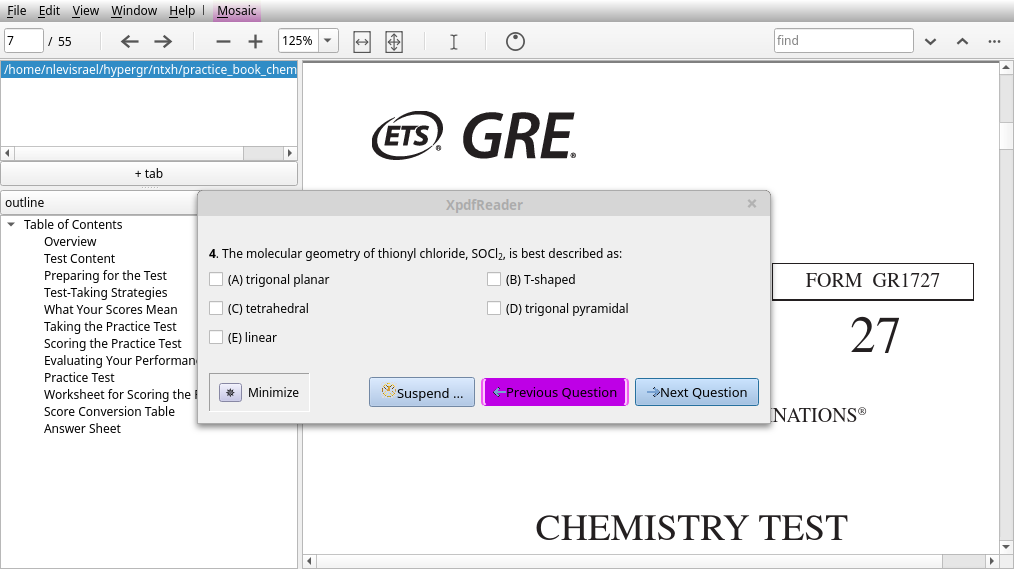
\includegraphics[width=110mm, 
    	trim={0mm 0 0 0mm},clip]
    	{ScreenShot.png}};

\curicon{4.4}{-1.44}

\end{tikzpicture}

\end{figure}

\mnote{Employing \EPF{} as test-taking software}
\p{One use-case for \EPF{} is to embed capabilities 
to host or administer tests within document viewers 
and scientific applications.  At the most basic 
level, these features include separate windows 
which show questions and answer choices, with 
options to navigate between questions.  When used 
for test preparation, students can use this format 
as a convenient simulation of an actual test, while 
also browsing back and forth between the question/answer 
window and the host application.  As depicted in 
Figure ~\ref{fig:i1}, question/answer plugins may 
be embedded in a \PDF{} viewer which loads a 
practice test in text format (in this case practice 
for the Chemistry \GRE{}), so students have the 
option of reading through the practice materials  
as a book-like publication and also conducting a 
practice test session in a more exam-like fashion, 
viewing one question at a time.}

\mnote{Writing exams with \LaTeX{} and \XPDF{} plugins.}
\p{To support 
this technology, \EPF{} distributions can include 
\LaTeX{} packages for composing exams which allow 
the questions and answers to be automatically 
extracted from the \TeX{} sources, packaged in a 
structured format (such as \XML{}), and placed 
as an embedded file in the generated \PDF{} document.  
This embedded data can then be read by 
\EPF{} plugins to create the question/answer windows.  
In documents (such as the \GRE{} practices) where 
questions are printed as part of the publication text, 
the \LaTeX{} code can store questions' \PDF{} coordinates 
so that the document automatically scrolls while 
students work their way through a practice test session.  
On the other hand, the same technology can be 
used to add review questions and answers to 
documents which are not expressly designed 
as test-prep materials, such as textbooks and 
research papers.  In this latter case, 
question/answer windows may be synced to 
sentences or paragraphs in the publication 
which are relevant to the review question that 
the student is currently reading in 
the question/answer window.}

\mnote{Remote Test Administration}
\p{Similar technology can also potentially be 
used for remote administration of actual 
exams.  Such a use-case is consistent with 
the current trend toward online test-taking --- 
a trend which may be accelerate in the near future 
as educational opportunities tick upward 
in remote areas where students cannot easily 
travel to testing centers (or even due to 
situations such as Covid-19 that disrupt 
conventional testing logistics).  Remote 
administration via \EPF{} is feasible if 
the plugins communicate students' answers 
in real time to \API{}s provided by the 
testing service.  Architecturally, the 
overall setup is then similar to 
online test-taking, except that students 
use technical applications or document viewers 
instead of web browsers for the actual test-taking.}

\mnote{How \EPF{} enables multi-application networking}
\p{In addition to potential test-taking features, \EPF{} 
also supports connecting multiple applications, 
so that students benefit from an interactive, multi-media 
pedagogical environment.  \lEPF{} refers not to a 
single plugin, but a 
toolkit for implementing ETS plugins to be 
embedded in many different applications.  
These plugins should be sufficiently similar 
that students or instructors familiar with an 
ETS plugin in one context (chemistry, for example) 
would quickly understand how to use plugins present 
in a different context.  An important \EPF{} feature 
is that distinct ETS plugins would be able to 
communicate with each other.  In particular, 
Document Viewer plugins would send data to 
plugins for scientific or multimedia applications so 
that students could access multimedia content 
linked to test-preparation materials.}


\p{\begin{wrapfigure}{r}{110mm}
		\caption{A Thionyl Chloride Question in XpdfReader}
\label{fig:tc}
\begin{tikzpicture}

\node[inner sep=0pt] (x1) at (0,0)
    {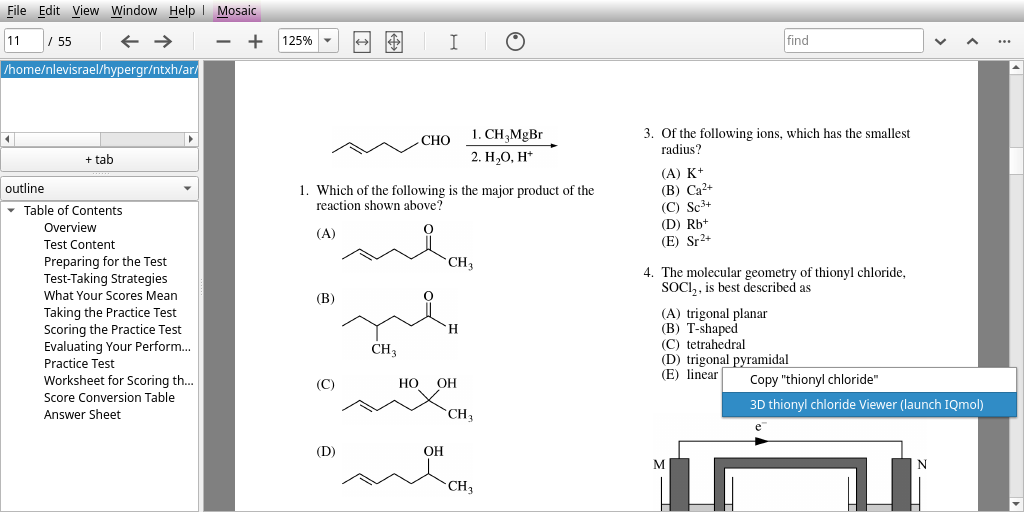
\includegraphics[width=110mm, 
    	trim={84mm 0 1mm 34mm},clip]
    	{xScreenShot2.png}};

\curicon{4.8}{-1.64}

\end{tikzpicture}


\end{wrapfigure}
For a concrete example of advanced functionality 
that can be achieved by connecting two distinct 
\EPF{} plugins, consider a student reading the \GRE{} 
Chemistry Practice Book published by ETS.  This book 
has sample questions such as (number 4, page 11) 
\textbf{The molecular geometry of thionyl chloride, 
SOCl$_2$, is best described as} \textit{(A) 
trigonal planar, (B) T-shaped, (C) tetrahedral, 
(D) trigonal pyramidal, or (E) linear}.
To understand 
this question/answer, it may help students to view a 
\ThreeD{} model of thionyl chloride, which can be done 
through molecular visualization software such as IQmol.  Accordingly, this specific question in the book 
may be associated with Molecular Data file for 
SOCl$_2$ (this file is available from the Chemical Abstracts Service database). \hspace{1em} The relation between the specific textual location  

\begin{wrapfigure}{l}{110mm}
	
%\begin{figure}[h]
\caption{Thionyl Chloride in IQmol}
\label{fig:i1}

\begin{tikzpicture}

\node[inner sep=0pt] (x1) at (0,0)
    {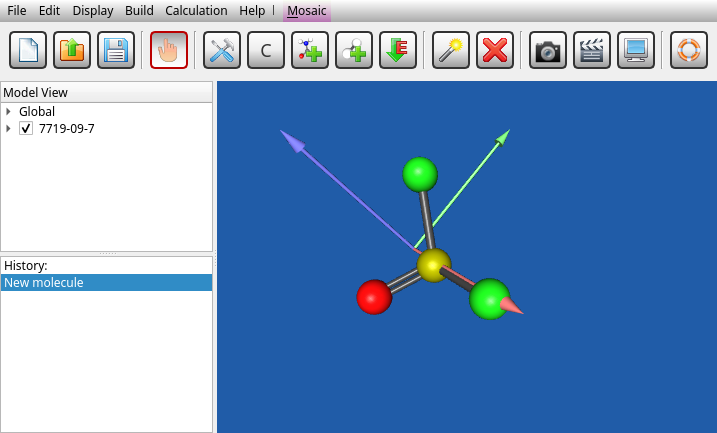
\includegraphics[width=110mm, 
    	trim={0mm 25mm 6mm 0mm},clip]
    	{iScreenShot1.png}};
    
%\curicon{0}{10}

\end{tikzpicture}
%\end{figure}

\end{wrapfigure}\noindent{}(where the practice Question 4 is 
presented) and the supplemental Molecular Data file 
would be asserted in the Document Infoset, and 
read by a document viewer (e.g., \XPDF{}).  The 
\XPDF{} plugin would then launch IQmol and send the 
molecular file to the IQmol ETS Plugin, with instructions 
to load this file into an IQmol session 
(see Figure ~\ref{fig:i1}).  The end result 
would be that the student, with a single 
click (such as selecting a visualization action from 
a context menu on the practice question) have access 
to an interactive \ThreeD{} graphic representing 
thionyl chloride.  (Of course, analogous 
functionality would be available for any chemical 
compound with multimedia files in formats 
like Molecular Data, Protein Data Bank, or Chemical 
Markup Language).}

\p{\begin{wrapfigure}{r}{110mm}
		
\begin{tikzpicture}

\node[inner sep=0pt] (x1) at (0,20)
    {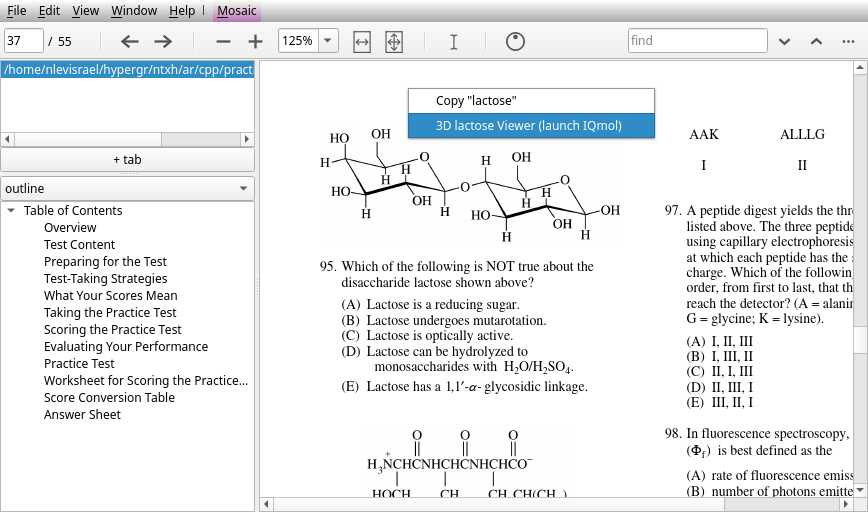
\includegraphics[width=110mm, 
    	trim={30mm 0 0 30mm},clip]
    	{xScreenShot1.png}};

\curicon{4.4}{-1.44}

%\node[inner sep=0pt] (x1) at (0,0)
%    {\includegraphics[width=110mm, 
%    	trim={30mm 0 0 30mm},clip]
%    	{iScreenShot2.png}};

\end{tikzpicture}


	\end{wrapfigure}
The data sent between \EPF{} applications 
may be more complex than a request to open 
a single multimedia file.  Suppose a student reading 	
the GRE Chemistry practice exam launches IQmol a 
second time --- perhaps in conjunction with a 
later question (95) about the molecular structure of 
glucose.  In this case, the plugin can send 
information not only about the present request but 
about the student's prior usage; in particular 
the fact that he or she had previously viewed the 
SOCl$_2$ file.  The \EPF{} plugin on the IQmol 
side can then load the prior file along with the 
new one, so the student can browse back to prior 
screens if desired (see the Model View panel on 
Figure ~\ref{fig:i2}).}
\begin{figure}[h]
\caption{Lactose in IQmol}
\label{fig:i2}

\begin{tikzpicture}

\node[inner sep=0pt] (x1) at (0,0)
    {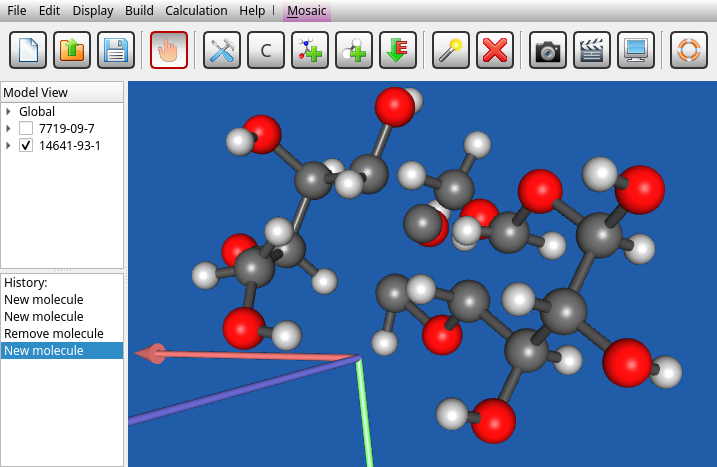
\includegraphics[%width=110mm, 
    	trim={0mm 0 0 0mm},clip]
    	{iScreenShot2.png}};

\end{tikzpicture}
\end{figure}


\p{\begin{wrapfigure}{l}{115mm}
		
\begin{tikzpicture}

\node[inner sep=0pt] (x1) at (0,0)
    {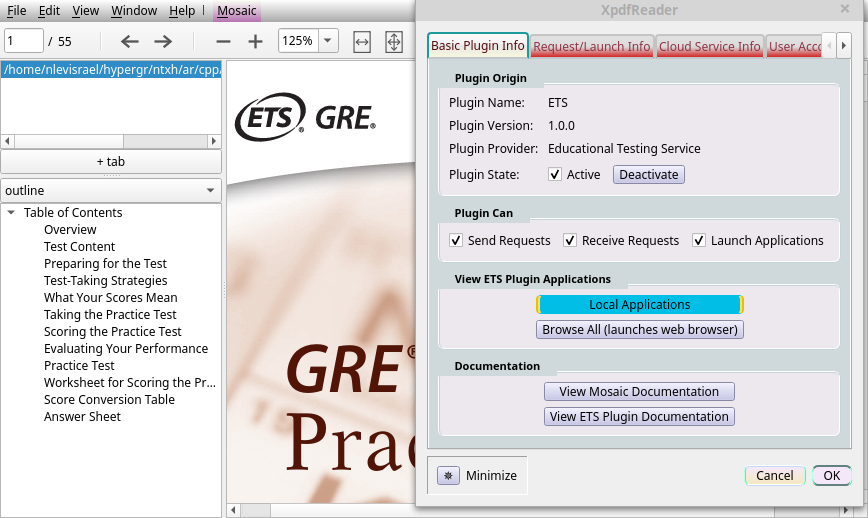
\includegraphics[width=115mm, 
    	trim={54mm 0 0 0mm},clip]
    	{xScreenShot.png}};

\curicon{3.4}{-1.34}

\end{tikzpicture}

	\end{wrapfigure}In general, the functionality 
	provided by each ETS plugin will 
	depend in part on the host application where the 
	plugin is embedded.  An IQmol plugin would load 
	cheminformatic files and may activate IQmol's analytic 
	capabilities in the domain of chemistry, whereas 
	a plugin in Data Visualization applications (such 
	as ParaView) could open quantitative data sets 
	with 2D or 3D views (via surfaces, scatter-plots, 
	bar charts, etc.) and activate statistical calculations.  Certain functionality, however, would be shared 
	among all ETS plugin, including a dialog window to 
	show basic plugin information (see figure at right) 
	and also a more detailed review of data transmitted 
	between applications via plugins.  
	The \q{request info} tab allows students, instructors, 
	and plugin developers to see information about the 
	request which caused the current application to be 
	launched or to open a specific file.}

\p{In addition to data visualization, scientific 
applications can help students understand concepts 
which are covered by a test.  For example, a later 
\GRE{} Chemistry practice question concerns 
Orbital Angular Momentum.  To understand 
this topic, students may benefit from hands-on 
experience calculating and visualizing 
Molecular Orbitals in IQmol.  In this 
scenario, once again, the practice book may 
be linked to IQmol through the Orbital Angular 
Momentum question.  However, in this case, 
instead of showing a single molecule, IQmol 
could load an interactive tutorial --- 
provided by the ETS Plugin --- explaining 
the Canonical Orbital Surfaces features in 
IQmol and enabling students to explore 
these with a variety of different molecules.}

\begin{figure}[h!]
\caption{Request Information in IQmol}
\label{fig:i6}

\begin{tikzpicture}

\node[inner sep=0pt] (x1) at (0,0)
    {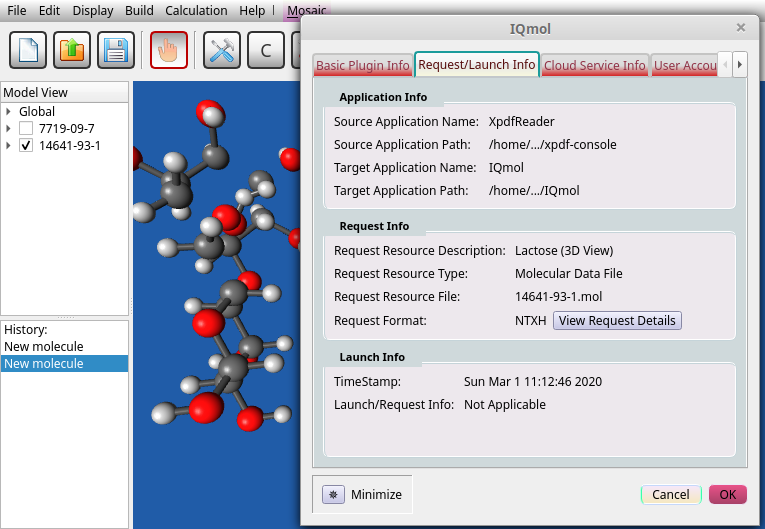
\includegraphics[width=\textwidth, 
    	trim={0mm 5mm 0mm 0mm},clip]
    	{iScreenShot.png}};

\curicon{8.2}{-6.1}

\end{tikzpicture}
\end{figure}


\vspace{2em}
\noindent\lun{Use-Cases for the Proposed ETS Plugin Framework}
{\sectsp}

\p{The above figures illustrate some of the 
canonical use-cases for ETS plugins: students 
read textbooks, articles, 
or test-preparation materials which are be enhanced 
with multimedia content.  For other use cases, consider 
the following scenarios: 
\vspace*{-2em}
\begin{mldescription}
\mlitem[Scenario 1: Using scientific 
application as pedagogical tools]  
Teachers often instruct students to download 
and install software relevant to the course curriculum, 
and this software can potentially be an essential 
part of the course content.  Instructors may 
(1) use the visualization capabilities of these 
domain-specific applications to help students 
understand the concepts covered in class; 
(2) provide instruction in how to use the 
software as part of the curriculum; 
(3) evaluate students' understanding of the 
software as part of their assessment of 
students' mastery of the curriculum; or 
(4) use applications' analytic features as an 
overview of analytic or quantitative methodologies 
relevant to the course's subject matter.  In 
the case of IQmol, features such as 
energy minimization, plotting orbitals, 
calculating vibrational frequencies, and many 
other chemphysical computations provide an 
overview of scientific concepts which 
might be covered in a Chemistry class. 

\mnote{Science applications as\\ teaching tools} 
\pseudoIndent{} To facilitate the 
use of scientific applications as teaching tools, 
\LPF{} plugins help instructors personalize the 
applications which their students use in 
conjunction with course curricula.  Again using IQmol as 
a case-study, an ETS plugin could show students a list of molecular 
examples discussed in class (based on data 
provided by the instructor) and allow students 
to view the corresponding \ThreeD{} molecular 
graphics accordingly.  

\mlitem[Scenario 2: Authors or instructors 
analyze publications' content to develop teaching 
materials]  When documents are read in an 
educational context, they become part of a 
larger ecosystem that extends beyond publication 
itself --- an ecosystem of assessment, test preparation, 
curricular design, and overall teaching environments 
(labs, classrooms, and so forth).  
%\mnote{Pedago\-gical use-cases for \LPF{}}
%Such use-cases illustrate the value of 
%machine-readable Document Infosets which provide 
%structured access to publication content, as opposed 
%to the merely visual access offered by \PDF{} files.  
Pedagogically using publications can involve extracting 
information from texts, or laying on additional 
content: inserting review questions at strategic 
points in the text; compiling glossaries indicating 
when technical terms are first used; foregrounding 
graphics and figure illustrations and encouraging 
students to explore them in depth 
(for instance, performing for themselves the calculations 
which are plotted in a statistical diagram; or 
identifying the axes, scales of measurement, dimensions, 
free and dependent parameters, and other mathematical 
details of a quantitative illustration).  Both of 
these kinds of operations --- extracting or adding 
content --- require computational access to a 
Document Infoset providing 
structured access to publication content.   
%Such use-cases illustrate the value of 
%machine-readable Document Infosets which provide 
%structured access to publication content, as opposed 
%to the merely visual access offered by \PDF{} files.   

\pseudoIndent{} Computer code which operates on 
manuscripts composed in coordination with 
\EPF{} can therefore act 
in consort with \EPF{} plugins.  For example, review questions 
or glossary definitions may linked to specific points 
in the text; this supplemental content may then 
be packaged along with the original publication.  
With suitable \EPF{} plugins, the document viewer 
can then process the review material and 
superimpose pedagogical questions, comments, or instructions 
on the underlying document text.     

\vspace{1em}
\mlitem[Scenario 3: Authors Develop Educational 
Materials Targeting Specific Applications]
In this scenario, authors compose books, articles, 
or test-preparation materials with the anticipation 
that readers will use specific software applications to 
enhance their reading experience.  This sort 
of interrelationship between publications and external 
software is presupposed at a rudimentary level 
as soon as authors link documents to specialized 
multimedia files.  For example, files in the 
ParaView Data (\PVD{}) format are intended to be 
used by the ParaView software; as a result, documents 
which reference such files presuppose that readers 
will have ParaView installed on their computer, for 
the full reading experience.  Similarly, files 
in cheminformatic formats such as Protein Data Bank 
(.pdb) or Chemical Markup Language (.cml) need to 
be opened with chemistry-related software like IQmol.  

%\mnote{Altering host applications via\\ plugins}      
\pseudoIndent{} Although it is not a prerequisite 
for \EPF{} plugins, one tool which can help 
authors customize their audience's reading 
experience is the Hypergraph Text Encoding 
Protocol (\HTXN{}), discussed in greater detail below.
\end{mldescription}
}

\vspace{1em}
\noindent\lun{The \lsHTXN{} Protocol}
{\sectsp}

\p{\lHTXN{} defines a protocol for (1) encoding manuscripts' 
character data and (2) defining document structures via 
graphs whose nodes correspond to 
ranges in a character stream.  
\lHTXN{} therefore uses 
\q{standoff annotation} (i.e., character 
encoding and document structure are 
defined in isolation from one another), and 
can be employed to encode manuscripts in 
many different markup formats.  
\lLXCR{} and \lHTXN{} are autonomous 
technologies (each may be used apart 
from the other), but they form a 
natural pairing, encompassing both 
the character/orthographic data and 
the document structure of 
manuscripts for publication.}

\mnote{\HTXN{} and multi-media content}  
\p{The central goal 
of \HTXN{} is to support the new generation of 
publishing technologies, where conventional 
document formats are increasingly being supplanted 
by digital, multimedia reader experiences.  
The conventional manuscript (the \q{primary} 
resource which is cited and downloaded) 
is, accordingly, often networked with a package of 
supplemental (or \q{secondary}) resources.  
\lHTXN{} is designed to 
rigorously document these multimedia networks, enabling 
e-readers and domain-specific applications to be 
integrated so that users may easily access multimedia content.}

\p{The generic term \q{multimedia content} actually 
encompasses multiple phenomena:

\vspace{-2em}
\begin{description}[leftmargin=2pt,
	labelindent=-2pt,labelsep=12pt]
\item[Multimedia Files]  Individual 
files representing audio, video, or 3D graphics content.  
These files may be linked from specific locations in 
the primary manuscript, or even embedded within manuscripts 
when they are published in \PDF{} format.
 
\item[Data Sets and Data Visualization]  Publishers 
increasingly emphasize sharing research data alongside 
texts, so readers can verify or even attempt to 
replicate claimed results.  Data sets are also a form 
of multimedia content because, apart from being aggregates 
of raw data, data sets are almost always accompanied 
by interactive, visual content: charts, diagrams, or 
plots to visualize the information holistically, or 
interactive tools to examine or navigate through the 
data set at finer scales.  

\item[Application Networks]  Another genre of multimedia 
content involves resources which may only be experienced 
through specialized software.  This classification encompasses 
content from particular scientific or technical domains, 
which is encoded in domain-specific formats: representations 
of molecular structures, archaeological sites, image-processing 
data, wave-forms for signal processing, sentence-parses for 
linguistic analysis, and so forth.  To conveniently access 
this kind of multimedia content, readers need to use software 
which can send signals to the specialized applications 
having the capability to recognize the domain-specific 
formats and translate them to interactive, 
visual presentations.  In short, publication viewers 
(e.g., e-readers) need to participate in multi-application 
networks, where data can be sent and received between 
each component.  One way to achieve this is via 
protocols, such as \LPF{}, shared between both e-readers and 
target applications.

\item[Publications-as-Applications]  In some 
cases, publications themselves are a form of 
multi-layered multimedia content.  This applies 
to publications which are not simply read from 
start to end, but instead naturally lend 
themselves to a reading process which navigates 
back and forth between different sections of 
the text, or juxtaposes different sections to be 
visible at the same time.  Testing materials 
and test preparation are a canonical example 
of such layered reading, where exam questions, 
instructions, supplemental materials (such 
as passages for reading-comprehension 
assessment), and comments or analyses about 
answers (in the case of prep materials) 
embody different layers which 
students may wish to view side-by-side.  
In these cases, e-readers cannot simply 
treat the publication as a single file.  
Instead, the manuscript needs 
to identify text segments which can be factored 
into different layers, and the e-reader 
needs to implement text-viewers which allow 
each layer to be viewed in separate windows, 
with readers able to juxtapose and position the 
windows as desired. 
\end{description}\vspace{-2em}
}


\p{\lHTXN{} represents publication manuscripts 
using structures which rigorously document 
publications' multimedia content and multi-application 
networking requirements.  This detailed 
multi-media support has several dimensions: 

\begin{enumerate}[leftmargin=2pt]
\inditem{} Defining points in the manuscript where 
multimedia files are linked or embedded: this 
involves annotating locations in the manuscript 
with hyper-references to multimedia files 
(audio, video, etc.) which readers should be 
able to access when they reach the corresponding 
point in the text.

\mnote{\HTXN{} cross-references to data-\\sets}
\inditem{} Establishing granular cross-references between 
publications and multimedia content: this is a 
more complex case where manuscript locations have to 
link \textit{to} or \textit{from} limited 
\textit{portions} of the corresponding multimedia 
resources.  For example, a passage in the manuscript 
may discuss a single sample within a data set; or 
may explicate a particular facet of the data set, 
such as an individual column in a tabular 
information space, or a specific set of 
statistical parameters against which quantitative 
operations are performed.  These scenarios 
call for bi-directional cross-references between the 
data set and the publication, wherein the granular 
data-set facet topically relevant to the 
corresponding manuscript location (the sample, 
table-column, parameters, etc.) is formally 
isolated and declared as a reference-target.  

\mnote{\HTXN{} cross-references to multi-\\media assets}
\inditem{} Cross-references may also be 
defined between publications' non-textual or 
non-paragraph content and corresponding 
multimedia resources.  For example, tables 
or diagrams visually presented in a manuscript 
may be liked to statistical data from which 
the figures are derived.  A similar situation 
applies when visuals included in a publication 
are linked to multimedia resources which 
represent the same information in a different 
experiential register: a \PDF{} document may 
include a two-dimensional graphic which is created 
by taking a camera shot of a \ThreeD{} model, 
which readers may also experience with a 
\ThreeD{} graphics engine; or a publication may 
reproduce a graph or scatter-plot derived 
from a data set, where data visualization 
software can represent the same information 
in a more interactive medium, with parameters 
plotted as curves or surfaces in a \ThreeD{} 
ambient space, or where systems are visualized 
as systems evolving over time.  
\end{enumerate}
}

\p{A summary of the \HTXN{} protocol,  
sample documents which compile to \HTXN{}-encoded 
text, and more information about plugins, 
are all available on request from 
Linguistic Technology Systems.}

%\vspace{2em}
%\noindent\lun{The Proposed ETS Plugin Framework}
%{\sectsp}



\end{document}


